\hypertarget{earlyexiting}{%
	\chapter{Early Exiting}\label{ch:earlyexit}}
\thispagestyle{fancy}

In this chapter we study accuracy latency trade-off of the early exiting \gls{dnn}s, by experimentation of exit thresholds and delay thresholds. We have found, that the early exiting have capabilities to better accommodate delay threshold, than conventional single-exit \gls{dnn}s. The chapter is structured as follows, section \ref{sec:ee-theory} present the theoretical background for early exit models. In section \ref{sec:ee-metrics} we define the metrics used in our experiments. In section \ref{sec:ee-exp-setup} we descibe our experimental setup. In Section \ref{sec:ee-implementation} we describe the implementation details of our early exiting models B-\gls{resnet} and B-\gls{densenet}. In section \ref{sec:ee-results} we present our results of training the models and experimenting with the fast inference framework using exit threshold and delay threshold. In section \ref{sec:ee-summary} we discuss our results.

\section{Theory} \label{sec:ee-theory}

Early exiting \gls{dnn} draws inspiration from another \gls{cv} algorithm, Viola-Jones \cite{viola_rapid_2001}. Viola Jones Face Detection was proposed in \citeyear{viola_rapid_2001}. The idea is a stacking or cascaded less accurate predictors to build a strong predictor. The predictors increasingly gain confidence when running the algorithm which termintates when the confidence has reached a threshold. Early exiting \gls{dnn} likewise stacks multiple classifiers. The \gls{dnn} can too be terminated, when a prediction with satisfying confidence is obtained. The early exit \gls{dnn} have shown promising results in \cite{leroux_cascading_2017, teerapittayanon_branchynet:_2016, leroux_resource-constrained_2015, teerapittayanon_distributed_2017, huang_multi-scale_2017, li_edge_2018}, and have primarily been used to solve two challenges in current literature.

\begin{enumerate}
	\item Reducing average inference latency and power consumption by letting samples prematurely exit the model based on random distributions \cite{bibid} or samples passing a threshold measure of confidence \cite{teerapittayanon_branchynet:_2016}.
	\item Comply with application time constraints by exit selection or sub-model selection. By only inference samples up to a selected exit possible to meet stringent delay constraints and reduce waste of computation \cite{li_edge_2018}. 
\end{enumerate}

Early exiting relies on the assumption, that the majority of samples are easy to classify correctly, and that \gls{dnn}s only have become deeper to accurately classify more difficult samples.

\begin{figure}
	\captionsetup[subfigure]{justification=centering}
	\centering
	\subfloat[bluetick]{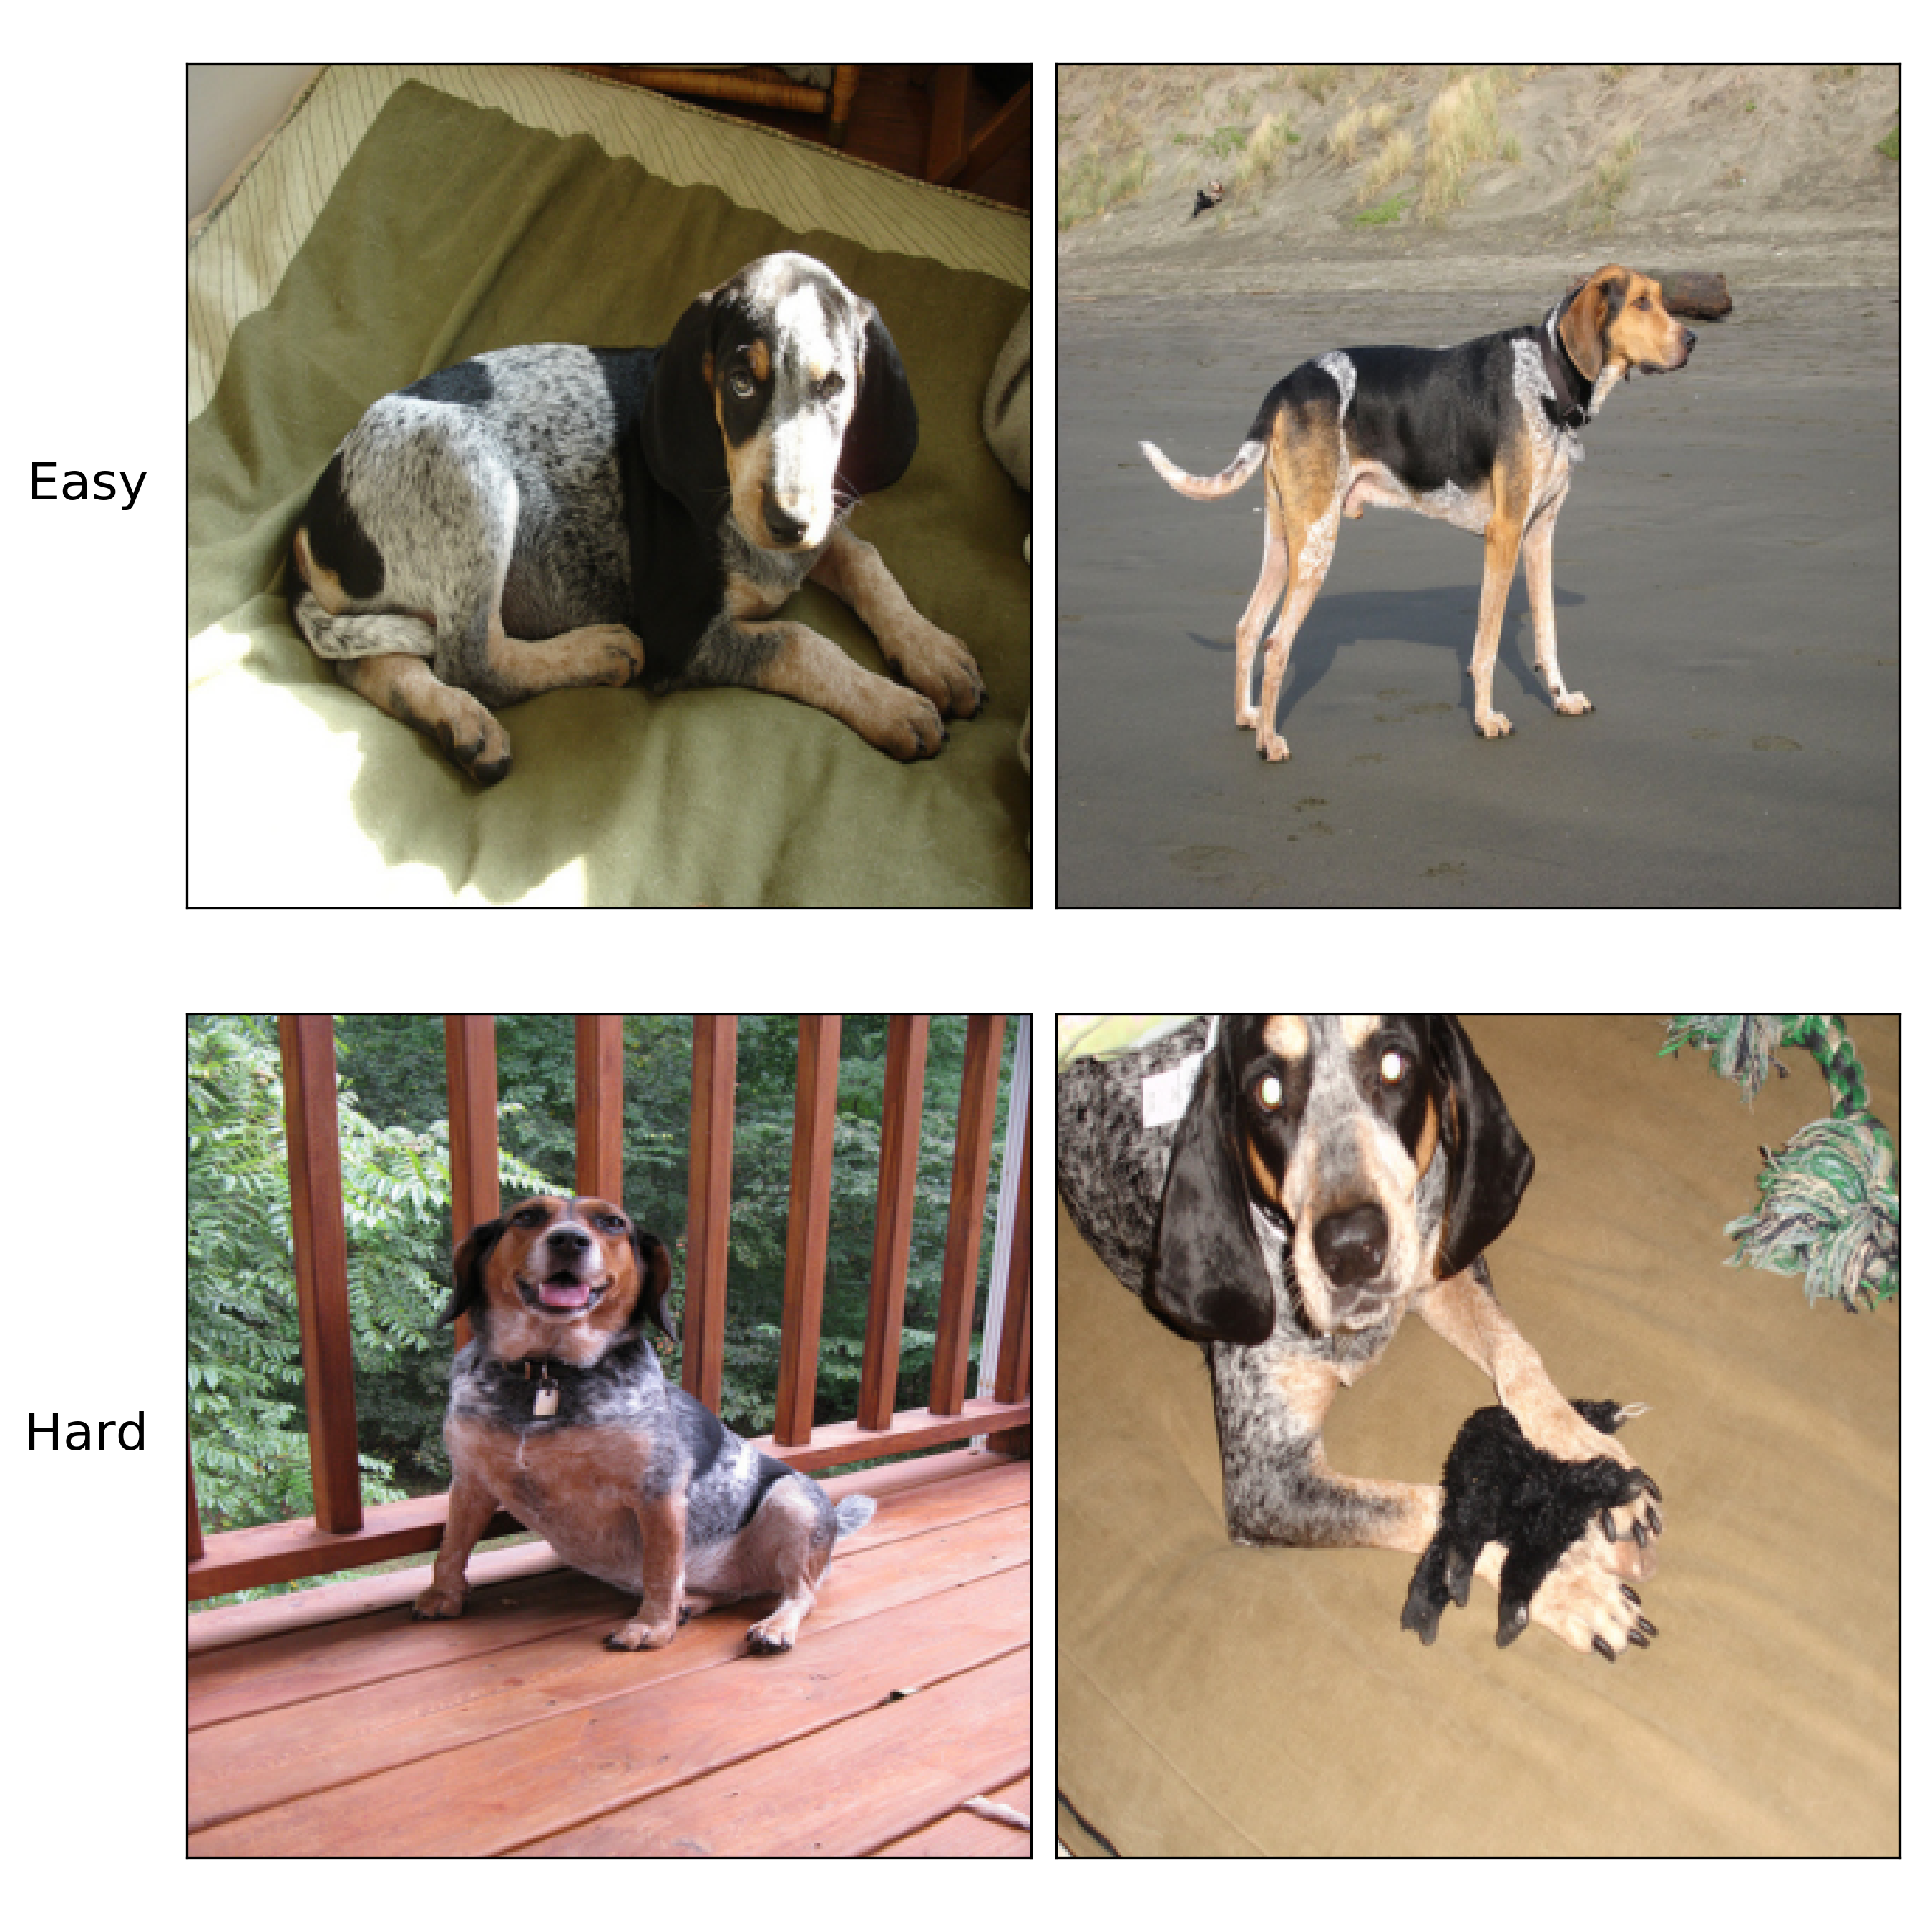
\includegraphics[width=0.5\linewidth]{figures/illustrations/hard_vs_easy_dog}}
	\subfloat[flamingo]{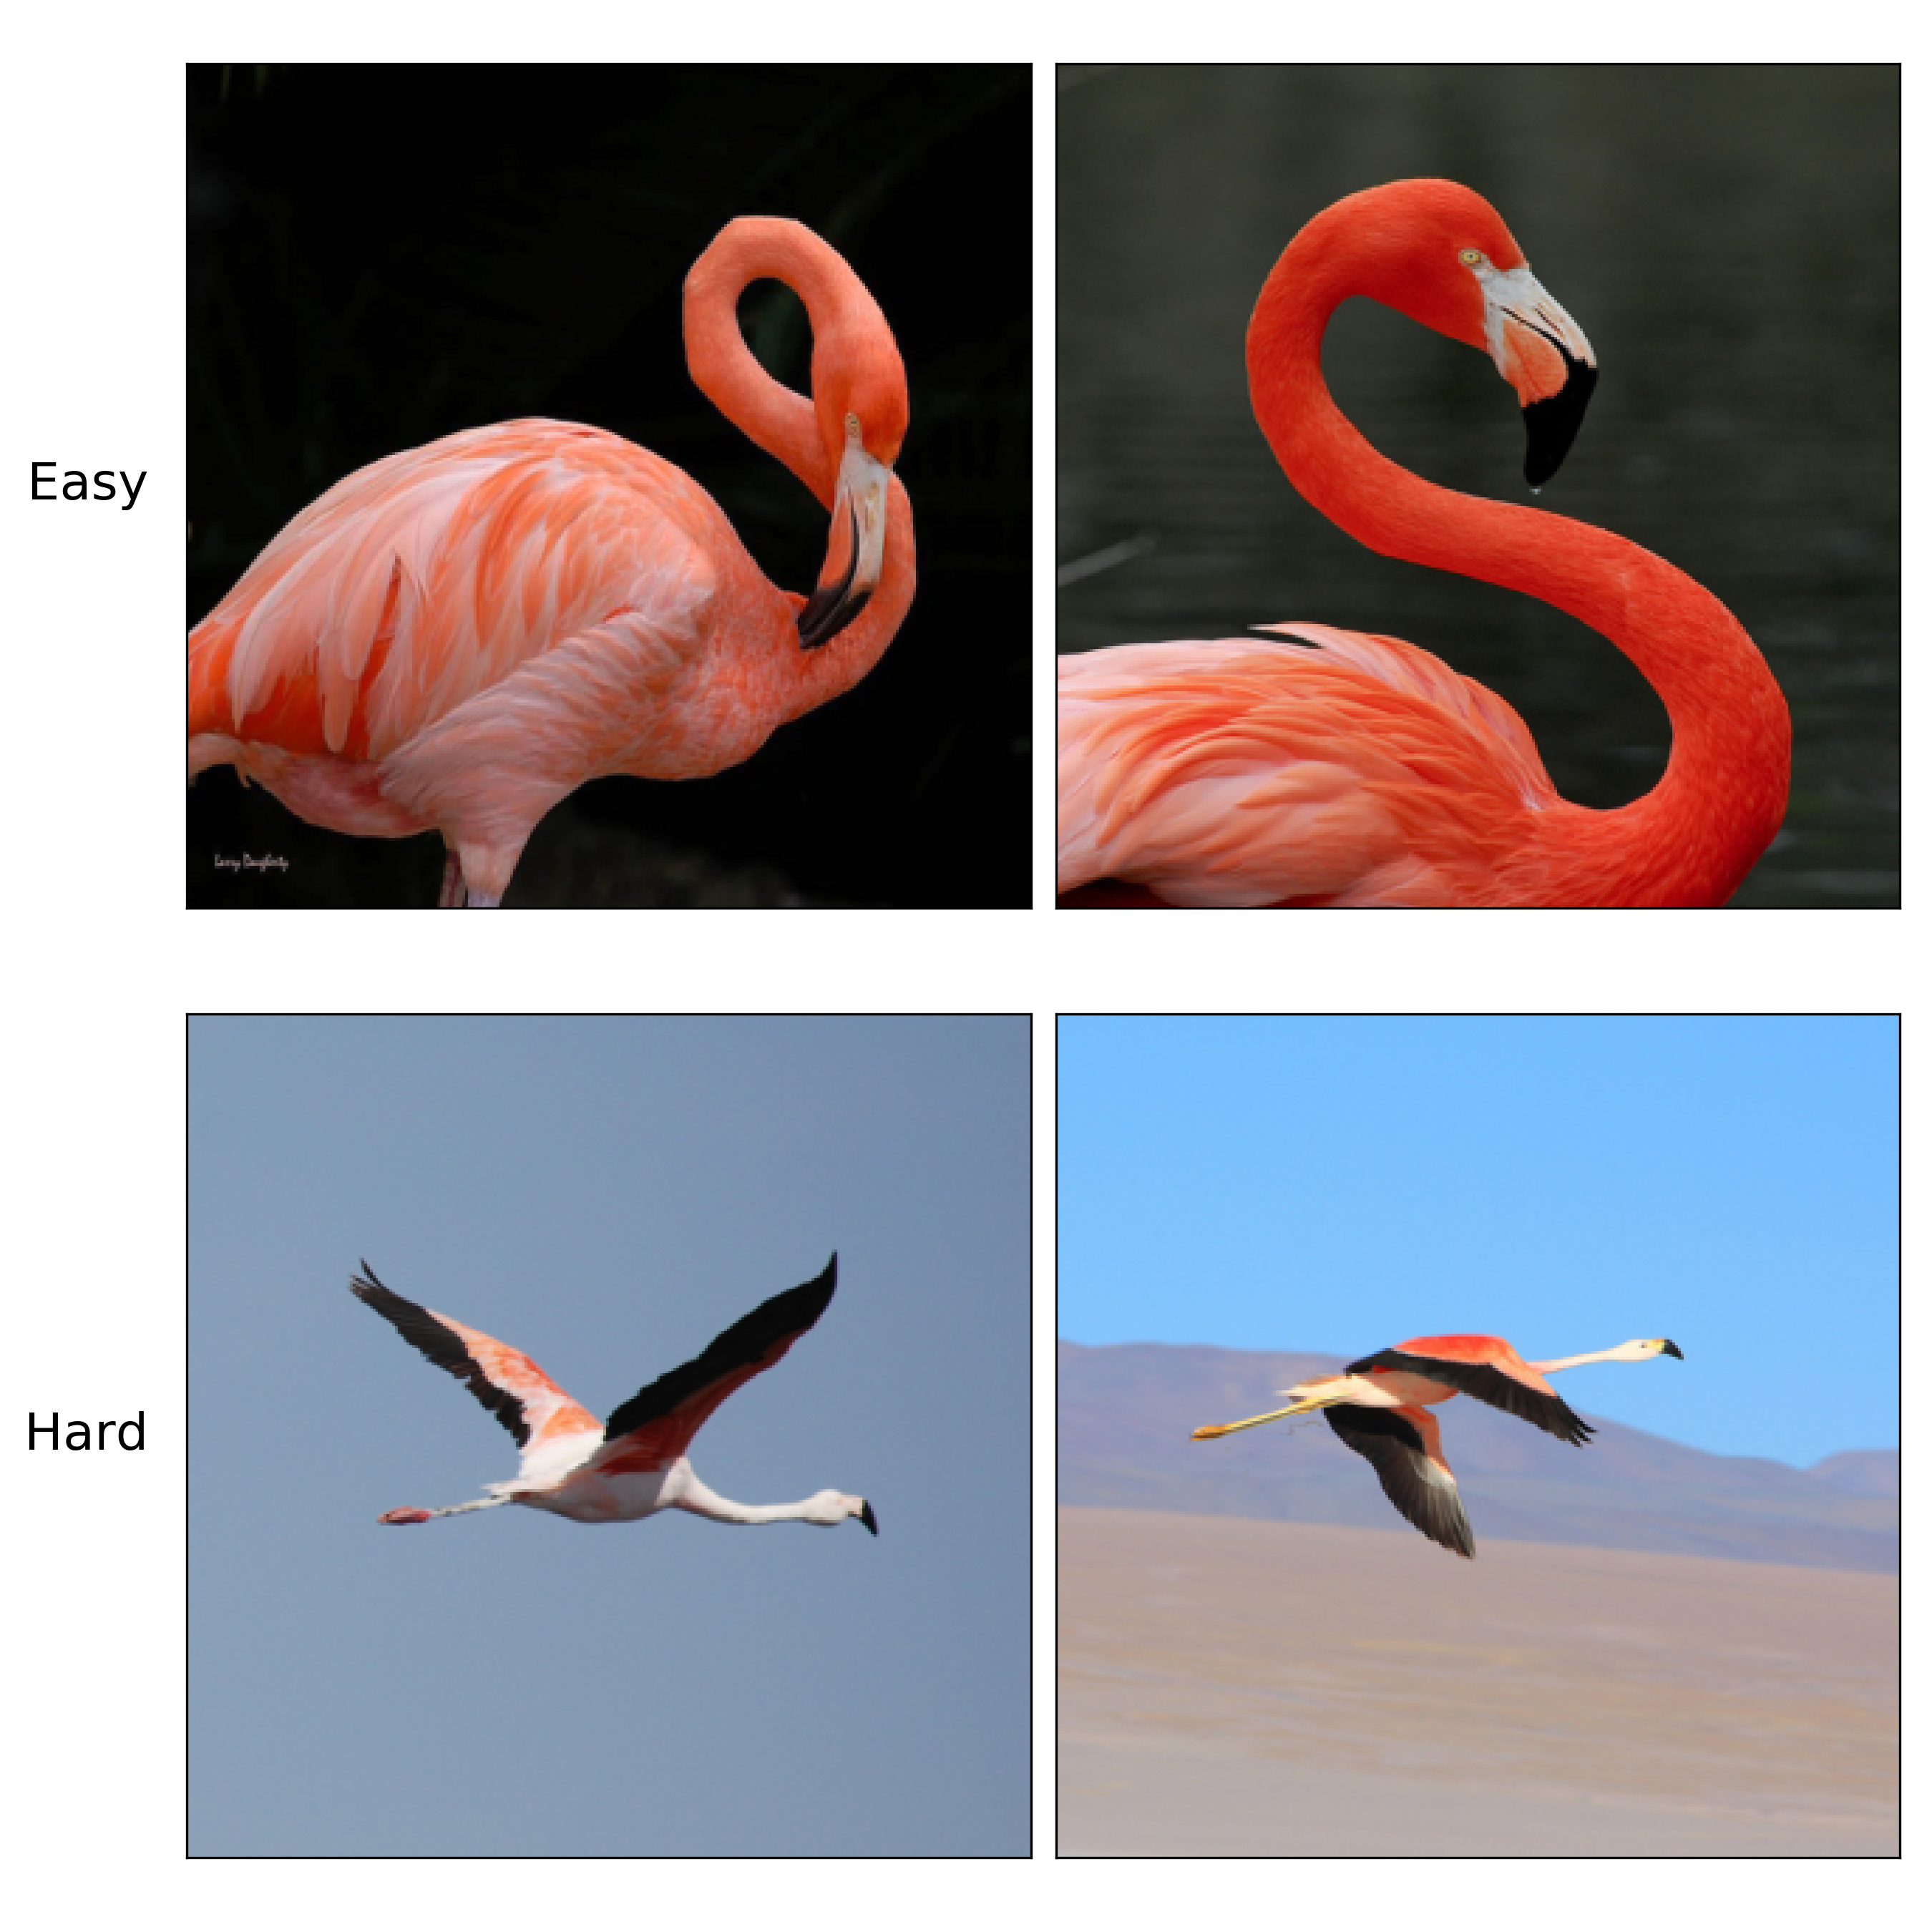
\includegraphics[width=0.5\linewidth]{figures/illustrations/hard_vs_easy_flamingo}}
	\caption[Easy vs. Hard Samples]{Easy vs. Hard Samples}
	\label{fig:hardvseasydog}
\end{figure}

As figures \ref{fig:hardvseasydog} exemplifies, samples where the object is easily separated from the background, are not occluded, and are viewed from angles which makes it easier to classify. Contrary samples that are not, are harder, additionally if the sample, should be discriminated from classes, with similar features are difficult such as different dog breeds etc. These examples have been found by running an early exit model. The hard examples have been found from looking at samples, that the \gls{dnn}s failed to classify, or can only classify using the last exit. The easy example are found by looking at samples, that can be correctly classified with high confidence by the first exit. 

\gls{branchynet} \cite{teerapittayanon_branchynet:_2016} and cascaded network \cite{leroux_resource-constrained_2015}, mentioned in \ref{label}, are both frameworks for constructing \gls{dnn}s with early exiting or stopping mechanisms. The difference between the two proposals are, cascaded network are seen as a general framework for adding intermediate classifiers after a layer, or a block of layers in a \gls{dnn}, wheres \gls{branchynet} construct early exit branches with additional layers, see figure \ref{fig:cascaded-vs-branchy}.

\begin{figure}
	\centering
	\subfloat[Branchy AlexNet, Source \citetitle{teerapittayanon_branchynet:_2016} \cite{teerapittayanon_branchynet:_2016}]{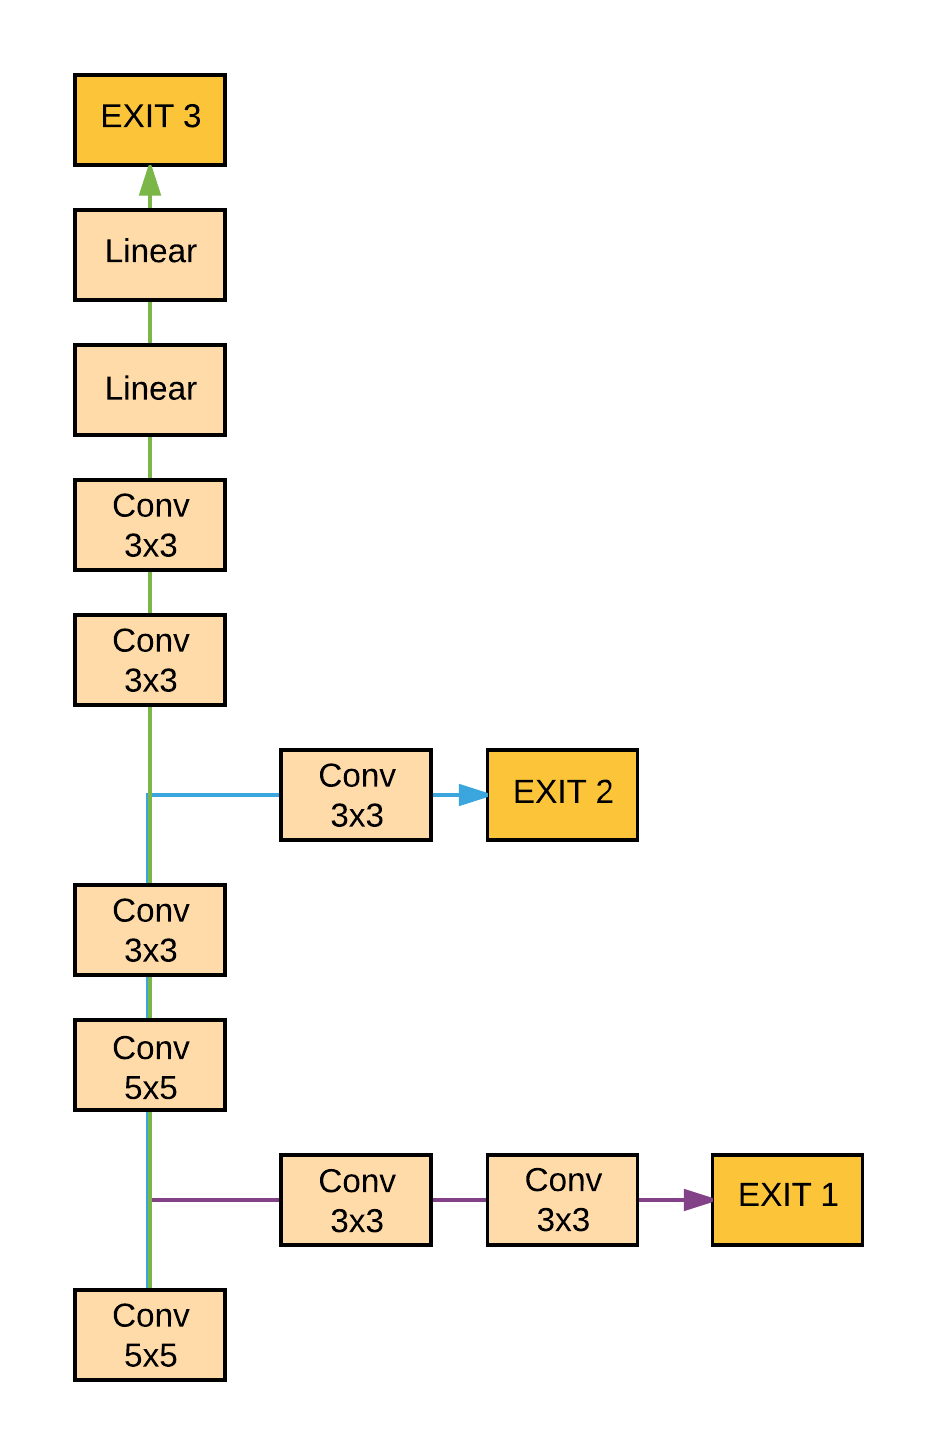
\includegraphics[height=.3\textheight]{figures/articles/branchynet}}
	\hspace{2em}
	\subfloat[Cascaded \gls{dnn}, Source \citetitle{leroux_resource-constrained_2015}\cite{leroux_resource-constrained_2015}]{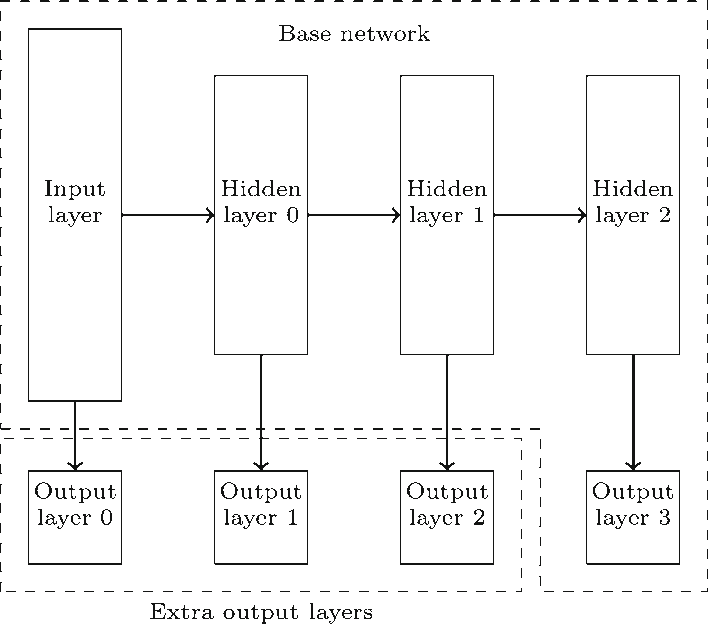
\includegraphics[height=.3\textheight]{figures/articles/cascade_dnn}}
	\caption[\gls{branchynet} vs. Cascaded \gls{dnn}]{\gls{branchynet} vs. Cascaded \gls{dnn}}
	\label{fig:cascaded-vs-branchy}
\end{figure}

\paragraph{Fast Inference Framework} The inference framework for the two proposal \gls{branchynet} and Cascaded \gls{dnn} is almost identical. A sample is inferred up to an exit and based on an exit criteria, it is decided to exit og continue the inference. The only difference is the choice of exit threshold. Cascaded \gls{dnn} uses the softmax score of the prediction, and evaluates if the score higher than a selected threshold, it is exited. \gls{branchynet} determines the entropy of the softmax output, and evaluates if the entropy is less a selected threshold, the sample is is is exited.

We use the fast inference framework defined in both \cite{leroux_resource-constrained_2015,teerapittayanon_branchynet:_2016}. However, we use two different score functions to evaluate, if the sample should be exited based on a threshold. The inference framework are written in pseudo code,  see listing \ref{lst:score-margin-inference}.

\begin{minipage}{\linewidth}
	\begin{lstlisting}[language = {}, mathescape=true, caption={Early Exit using Score-margin }, label={lst:score-margin-inference}]
procedure $\textsc{EarlyExitFastInference}$$(x, T )$
	for $k = 1\dots K$ do
		$z = f_{exit_k}(x)$
		$ \hat{y} = softmax(z) $
		if $$\hat{y}$ > T_k$ then
			return $\arg \max \hat{y}$
	return $\arg \max \hat{y}$ 
	\end{lstlisting}
\end{minipage}

\paragraph{Training Framework} 
Training cascaded \gls{dnn}, in \cite{leroux_resource-constrained_2015} it is proposed to train a network using a single end classifier. Once the model has convergence, the weights of the network are frozen and intermediate classfiers are attached, equivalent to use a pre-trained model and convert it to a cascaded models and train the entire network for a single epoch before freezing the network weights. The next phase is training all intermediate classifiers. The approach was tested and gave unsatisfactory results, see \ref{sec:training-results}. However, this particular method may work on datasets with small image sizes such as \gls{mnist} or \gls{cifar10}. Both \cite{leroux_resource-constrained_2015} and \cite{teerapittayanon_branchynet:_2016} uses the \gls{mnist} and \gls{cifar10} datasets. One may argue, that the two datasets used are not applicable to real-life scenarios, as the images are only 32x32 pixels and the datasets only contain 10.000 samples. In \cite{leroux_cascading_2017}, the follow-up paper to Cascaded \gls{dnn}, they train a frozen base network on the ImageNet dataset, but does not achieve particularly high accuracy on early exits.  

The \gls{branchynet} approach is remarkably similar. In \cite{teerapittayanon_branchynet:_2016} they define the \gls{branchynet} loss function, as an adaptation of the widely used softmax cross-entropy loss function.
\begin{align}
L\left(\mathbf{y},\hat{\mathbf{y}}\right) = - \frac{1}{C} \sum_{j =1}^{C} y_c \log \hat{y}_c
\end{align}
Where $ \bm{y} $ is a on-hot encoded ground truth vector, $ \bm{\hat{y}} $ is the output score vector of the softmax classfier and $ C $ is the number of class labels $ (1, 2, c, \dots, C) $.
	
The \gls{branchynet} loss function is defined as the weighted sum of the softmax cross-entropy loss of each branch-prediction. 

\begin{align}
	L_{\mathrm{BranchyNet}}(\hat{\mathbf{y}},\mathbf{y};\theta) = \sum_{n=1}^{N} w_n L \left(\hat{\mathbf{y}}_{n},\mathbf{y};\theta\right)
\end{align}

Where $ \bm{\hat{y}} $ is the output score vector of exit $ n $, $ w_n $ is the weight for exit $ n $ and $ \theta $ represents the parameters of the layers from an entry point to the exit point $ n $.

They claim, that the joint-optimization of multiple exits provides a regularization effect, thus countering over-fitting and potentially improves test accuracy. Additionally is also mitigates vanishing gradient, due to additional gradient signal from the early exits, which promotes more discriminative feature in early layers. In \gls{googlenet} \cite{szegedy_going_2015} auxiliary classifiers are too place in the middle of the network to counter vanishing gradients. However, that is also the only purpose for the auxiliary classifiers og \gls{googlenet}, as they are only used when training the network, hence no samples can exit the inference process prematurely. 

They have also too found, that first training the network end-to-end or using a pre-trained model, and then attach the intermediate exits/classifiers both improves the performance and shortens the training time. However, they do not suggest freezing the features of the networks. We have tried both freezing and unfreezing the network base and have found, that training the entire model is the far superior approach. 

 In the next section we describe the mathematical models used to evaluate the latency, accuracy and early exiting capabilities using confidence and delay thresholds.

\section{Metrics} \label{sec:ee-metrics}

Assume $ K $ denotes the number of image classes, $ N $ denotes the number of the exit points in a DNN, $ I $ denotes the number of images.
	\begin{enumdescript}
		\item[Latency Model] We adapt the same notation for the early exiting inference model and the conventional inference model with a single exit at the end of the \gls{dnn}. The \gls{dnn}s are build of blocks and classifiers.
		
		Assume:
		\begin{itemize}
			\item $T_{i,n}^{block}$ denotes the runtime inference an image $ i $ to the $ n $th block of the \gls{dnn} $ i $ for $ \left(1\leq n \leq N, 1 \leq i \leq I\right) $
			\item $T_{i,n}^{exit}$ denotes the runtime of the exit $ n $  to process image $i$ for $ \left(1\leq n \leq N, 1 \leq i \leq I\right) $
		\end{itemize}
		\begin{enumdescript}
			\item[Conventional Inference Model] The conventional inference model only have a single exit at block $ N $, hence all $ N $ blocks of the \gls{dnn} must have inferred the image $ i $ before $ i $ i classified at exit $ N $. Thus the latency model for a conventional inference model is presented as
			\begin{align}
			T^{ci}_{i,N}= \sum_{j=1}^{N} \left(T_{i,n}^{block}\right) + T_{i,N}^{exit}
			\end{align}
			\item[Early Exit Inference Model] The early exit inference model is adaptive. The inference of image $ i $ can terminate at any exit $ n $. If the classification exits from exit point $ n $, then the latency model for early exit inference model is presented as
			\begin{align}
			T_{i,n}^{ee}=\sum_{j=1}^{n} \left(T_{i,n}^{block} + T_{i,n}^{exit} \right) 
			\end{align}
			The additional classifiers of the early exit inference model add a overhead compared to the conventional inference model, however it may not be required to run all $ n $ blocks and classifiers of the early exiting inference model. 
		\end{enumdescript}
		
					
		
		\item[Accuracy Model] The accuracy model is independent of conventional or early exiting inference model. 
		
		Assume
		\begin{itemize}
			\item $ \mathbf{\hat{y}}_{i,n} = \left[\begin{array}{cccc}\hat{y}_{i,n,1} & \hat{y}_{i,n,2} & \dots & \hat{y}_{i,n,K}\end{array}\right] $ denotes the output score vector from the softmax classifier at exit point $ n $ for image $ i $
			\item $ \hat{y}_{i,n,k} $ denotes the score of class $ k $ from exit point $ n $ by processing image $ i $
				
			\end{itemize}
		\begin{enumdescript}
			\item[Prediction] The prediction of image $ i $ from the exit point $ n $ is denoted $ \hat{y}^*_{i,n} $ and will be
			\begin{align}
			\hat{y}^*_{i,n} = \arg \underset{n}{\max}\: \mathbf{\hat{y}}_{i,n}
			\end{align}
			Note that the prediction to go through the entire \gls{dnn} is $ \hat{y}^*_i  = \hat{y}_{i,N} $, i.e. the last exit $ N $ of the early exit model, or equivalent to the prediction of conventional inference model.
			
			\item[Accuracy] Assuming the ground truth of image $ i $ is $ y_i$ a class label taking values of $\left(1, 2, k, \dots, K \right) $. The inference accuracy of exit point $ n $ can be expressed by
			\begin{align}
			\bar{A}_{n}=1-\frac{1}{I} \sum_{i=1}^{I} \mathbb{I}\left(\left|\hat{y}_{i,n}-y_{i}\right|\right)
			\end{align}
			where $ \mathbb{I(\cdot)}  $ is a indicating function defined by
			\begin{align}
			\mathbb{I}(a)= \begin{cases}
			0, & \mathrm{if\:} a \leq 0, \\
			1, & \mathrm{otherwise}
			\end{cases}
			\end{align}
			We sum the number of errors or misclassifications. When $ \hat{y} \neq y $ our indicating function return a 1. The determine the probability of misclassification as, the number of errors divided by the total number of images. To convert into accuracy we subtract the error probability from 1.    
			
			
			
		\end{enumdescript}
	
		\item[Early Exit Condition] we define an early exit condition based on the output vector from the softmax classifier $ \bm{s}_{i,n} $ for image $ i $ at exit point $ n $. An image $ i $ is allowed to exit the model at exit point $ n $, if a score threshold $ \gamma_n $ at exit $ n $ is surpassed.
		
		Assume
		\begin{itemize}
			\item $ \bm{\gamma} = \left[\begin{array}{cccc}
			\gamma_{1} & \gamma_{n} & \dots & \gamma_{N} \end{array}\right]  $ denotes the threshold vector at exit point $ n $. It is seen in \cite{teerapittayanon_finding_2018}, that finding different threshold values for the exits can improve the accuracy. However, in our experiments, we have set $ \gamma_{1} = \gamma_{n} = \dots, = \gamma_{N}  $, as we are more concerned with latency. Evidently selecting a higher threshold value at an early exit, will cause less samples to exit and promote the use a later exit, which will cause additional inference delay.
		\end{itemize}
		
		We use two different score functions, the score-max $ f_{max}(\cdot) $ and the score-margin $ f_{margin} $, to evaluate against the threshold $ \gamma $. 
		
		\begin{enumdescript}
			
			
			\item[Score-Max] the score-max function $ f_{max}(\cdot)$ also used in \cite{leroux_resource-constrained_2015}, is a simple function, that takes the score vector $ \bm{s}_{i,n} $ of image $ i $ at exit $ n $ as input and outputs the maximum value of the vector. We express it as 
			\begin{align}
			f_{max}\left(\bm{\hat{y}}_{i,n}\right) = \max \bm{\hat{y}}_{i,n}
			\end{align}
			
			
			\item[Score-Margin] the score-margin function $ f_{margin}(\cdot)$, is defined and used in \cite{park_big/little_2015}- However, used for model selection and not early exiting. The function also takes the $ \bm{s}_{i,n} $ as input and returns the difference between the two largest elements. We express it as
			
			\begin{align}
			f_{margin}\left(\bm{\hat{y}}_{i,n}\right) = \hat{y}_{i,n}^{1st} - \hat{y}_{i,n}^{2nd}
			\end{align}
			where $ \hat{y}_{i,k}^{1st} $ denotes the largest element of $ \bm{\hat{y}}_{i,n} $ 
			and $ \hat{y}_{i,n}^{2nd} $ the second largest element of $ \bm{\hat{y}}_{i,n} $.
			
			
		\end{enumdescript}
		
		
		We express the probability of early exit, given the score function. For notation simplicity we write $ f_{\phi} = \{f_{max}, f_{margin}\}$, meaning we can choose to use either function. 
		\begin{align}
		\overline{F}^{exit} = \frac{1}{I}\sum_{i=1}^{I} \mathbb{I} \left(\gamma-f_{\phi}\left(\hat{y}_{i}\right) \right)
		\end{align}
	
	\item[Reliability Model] as we are concerned with time-sensitive real-time applications and services. We define a latency threshold $ \delta $. We have a delay violation if $ T_i \leq \delta $, hence the model have not provided a prediction within the time frame.
	
	\begin{enumdescript}
		\item[Timeout Probability]  We define the probability of timeout, the amount of samples not able to meet the delay requirement out of all samples.
		
		\begin{align}
		\overline{F}^{to}=\frac{1}{I}\sum_{i=1}^{I} \mathbb{I}\left(T_{i}-\delta\right)
		\end{align}
		
	\end{enumdescript}

	No we can formulate or reliability model, as the obtainable accuracy times the amount of samples able to meet the latency constraint.
	
	\begin{align}
	R= \bar{A} \cdot (1-\overline{F}^{to})
	\end{align}
	
	\item[Problem formulation] we can formulate our problem, as maximization of the accuracy with a time constraint. The inference time of image $ i $, cannot be greater than or equal to $ \delta $, our latency threshold. 
	
	\begin{maxi}
		{}{\bar{A}}
		{}{}
		\addConstraint{T_i}{\leq \delta}
	\end{maxi}
	
		
	\end{enumdescript}


Coherence \todo{add an outro to ease into next section}


\section{Implementation} \label{sec:ee-implementation}

\subsection{Branchy-ResNet} 

In this section is the residual layers, the building block of the residual network, is explained. Followed by a design description of Branchy-\gls{resnet}.

The depth of \gls{dnn} is of paramount importance to extract increasingly richer features from images to obtain highly accurate classification models cite{who}. Training very deep models with more than ten layer for convergence is not easy due to vanishing/exploding gradients. Residual Networks or \gls{resnet} \cite{he_deep_2015} have for long been a state-of-the-art network and won ILSVRC15 using up to 152 layers. The network is build of residual blocks, a \gls{dnn} layer designed for extremely deep networks. 

Just as plain \gls{vgg} nets, residual networks is still a stacking of  convolutional layers. The \gls{resnet}, however, adds a shortcut connection, which skips a layer or a block of layers. The skip connection adds the identity of input to the output of the layers/block, see figure \ref{fig:residualblock}

\begin{figure}
	\centering
	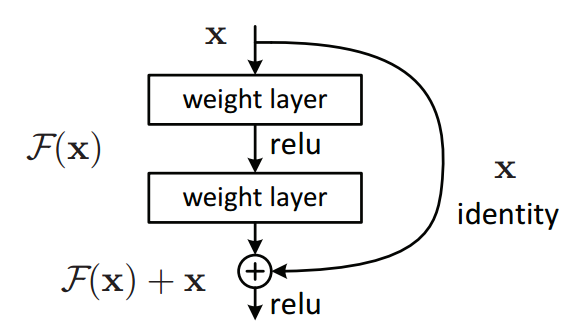
\includegraphics[width=.5\linewidth]{figures/models/residualblock}
	\caption[Residual Block]{Residaul Block}
	\label{fig:residualblock}
\end{figure}

Information from earlier layers are preserved by the residual, which diminishes the vanishing gradient problem. Thus this type of network have shown to be easier to train compared to it’s plain counterpart and able to obtain superior accuracy.  

Very deep residual networks comprised of up to 152 layers have also shown to be far more efficient requiring less \gls{flop}s, than \gls{vgg}16 comprised of only 16 layers, by introducing a bottleneck unit. The bottleneck reduces the dimensions by a $1 \times 1$ convolution, followed by a $3 \times 3$ convolution and then restoring the dimensions using a $1 \times 1$ convolution. \todo{fact check this!!}

The residual networkds proposed in \cite{he_deep_2015} are grouped into 4 resolutions block each of which downsamples the input data. The network are proposed with different number of layers (18, 34, 50, 101, 152) depending on the depth of the network. Table \ref{tbl:resnet101} describes the blocks and layers of the \gls{resnet} architecture. \gls{pytorch} provide implementations of these networks. The implementations can be trained from scratch or can be initialized with downloadable pretrained weights based on ImageNet. \gls{resnet}101 have been chosen for this project, as it has comparable depth to the smallest available \gls{pytorch} \gls{densenet}-121 implementation and also have similar inference latency on a Titan Xp (8.90ms and 8.93ms) \cite{bianco_benchmark_2018}.

\begin{minipage}{\linewidth}
\begin{longtabu}{>{\bfseries}X|X[c]|X[2c]}
	\caption[\gls{resnet}101 description]{\gls{resnet}101 description. The table describes the blocks of \gls{resnet}101, the size of the block and the layers of the block.} \label{tbl:resnet101} \\
	\toprule
	\rowfont{\bfseries}
	Resolution block & Output size & Layer description \tabularnewline
	\hline
	\endfirsthead
	\multicolumn{3}{@{}l}{\textbf{\textcolor{black}{Table \ref{tbl:resnet50}:}} continued}\\
	\toprule
	\rowfont{\bfseries}
	Conv block & Output size & Layer description \tabularnewline
	\hline
	\endhead % all the lines above this will be repeated on every page
	\hline
	\multicolumn{3}{@{}l}{continued \ldots}\\
	\endfoot
	\hline
	\endlastfoot
	conv1 & $112\times 112$& $7\times 7, 64, \:\mathrm{stride}\: 2$ \tabularnewline \hline
	
	\multirow{5}{*}{conv2\_x} 	& \multirow{5}{*}{$56 \times 56$} 	& $3 \times 3 \:\mathrm{maxpool, stride}\: 2 $ \\ \tabucline{3-3} & & \multirow{4}{*}{
		$\begin{bmatrix}
		1 \times 1, 64 \\ 3 \times 3, 64 \\1 \times 1, 256
		\end{bmatrix} \times 3$ }		\tabularnewline										
	& & 	\tabularnewline
	& & 	\tabularnewline
	& & 	\tabularnewline
	\hline
	
	\multirow{4}{*}{conv3\_x} 	& \multirow{4}{*}{$28\times 28$} & \multirow{4}{*}{
		$\begin{bmatrix}
		1 \times 1, 128 \\ 3 \times 3, 128 \\1 \times 1, 512
		\end{bmatrix} \times 4$ }		\tabularnewline										
	& & 	\tabularnewline
	& & 	\tabularnewline
	& & 	\tabularnewline
	\hline
	
	\multirow{4}{*}{conv4\_x} 	& \multirow{4}{*}{$14\times 14$} & \multirow{4}{*}{
		$\begin{bmatrix}
		1 \times 1, 256 \\ 3 \times 3, 256 \\1 \times 1, 1024
		\end{bmatrix} \times 23$}		\tabularnewline										
	& & 	\tabularnewline
	& & 	\tabularnewline
	& & 	\tabularnewline
	\hline
	
	\multirow{4}{*}{conv5\_x} 	& \multirow{4}{*}{$7\times 7$} & \multirow{4}{*}{
		$\begin{bmatrix}
		1 \times 1, 512 \\ 3 \times 3, 512 \\1 \times 1, 2048
		\end{bmatrix} \times 3$}		\tabularnewline										
	& & 	\tabularnewline
	& & 	\tabularnewline
	& & 	\tabularnewline
	\hline
	
	Classifier & \multicolumn2{c}{$\mathrm{Avg.\: Pool,\:} 1000d\: \mathrm{fc,\: Softmax}$} \tabularnewline
	\bottomrule
\end{longtabu}
\color{caption-color}{\textit{Source: \citetitle{he_deep_2015}, by \citeauthor{he_deep_2015} \cite{he_deep_2015}, describes a full list of Residual Networks (\gls{resnet}18, \gls{resnet}34, \gls{resnet}50, \gls{resnet}101 and \gls{resnet}152)}}\color{main-color}
\end{minipage}

The early exits of B-\gls{resnet}101 is placed immediately after a resolution block, as;
\begin{enumerate}
	\item The exit must be placed sufficiently deep, so that the model is actually able to correctly predict some input samples
	\item If used in a collaborative setup, a smaller feature representation is desired. The exits are placed after the resolution block, as the filter size is unchanged within the block. 
\end{enumerate}
To contruct the early exits a pooling-layer followed by a fully-connected linear classifier is added. Figure \ref{fig:b-resnet} illustrates the early exiting model B-\gls{resnet}101.

\begin{figure}
	\centering
	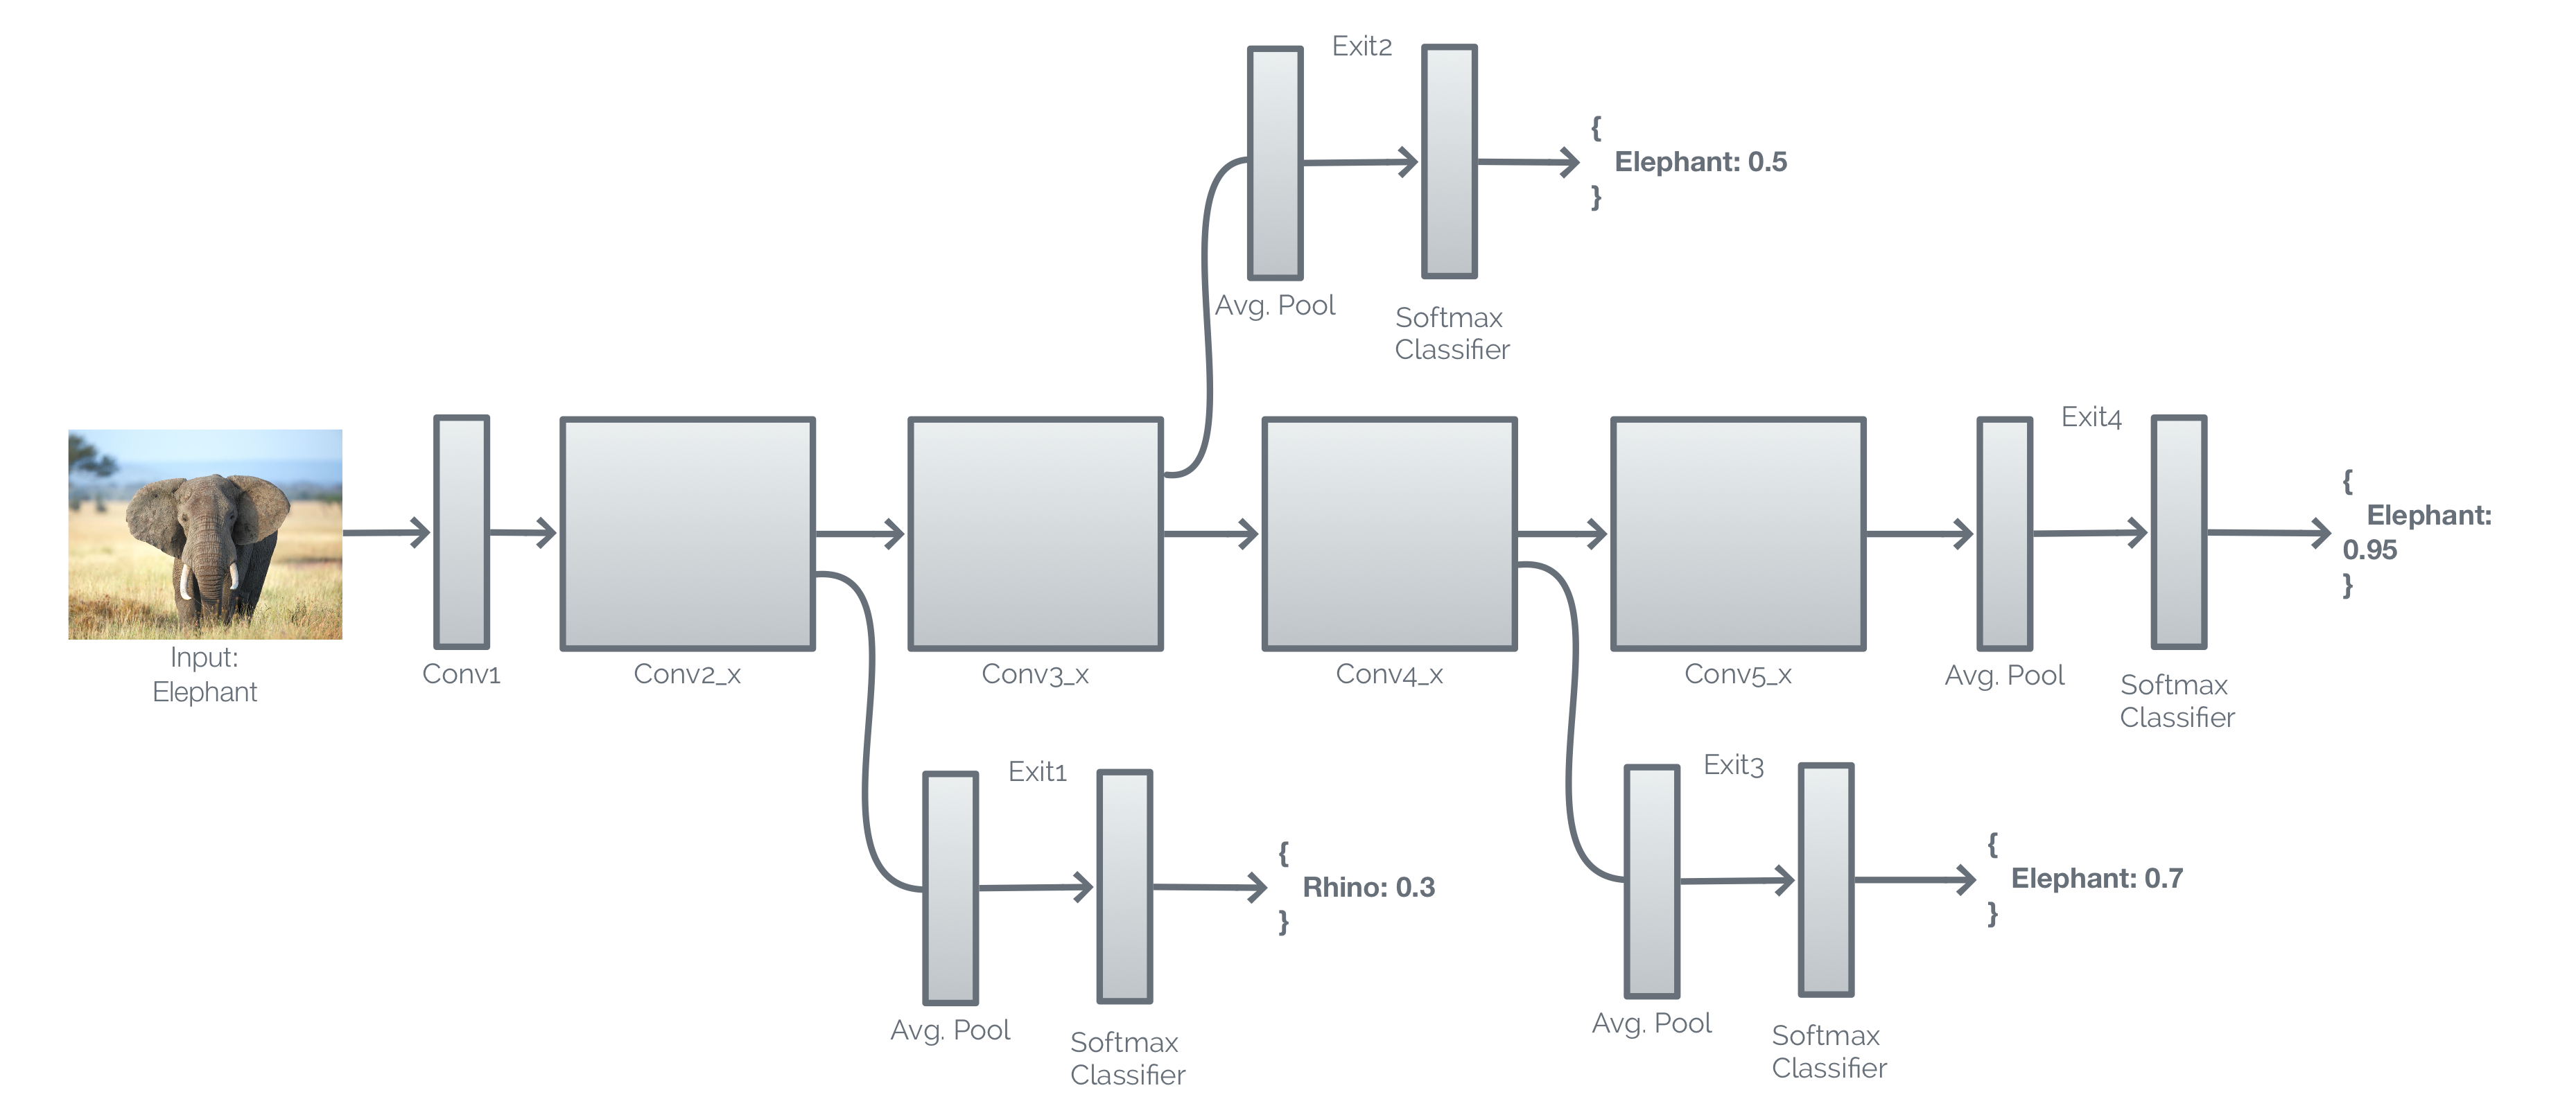
\includegraphics[width=\linewidth]{figures/models/BResNet}
	\caption[B-\gls{resnet} architecture]{Branchy-\gls{resnet}101: \gls{resnet}101 extended to implement the BranchyNet framework. The figure illustrates how classification confidence grows, as we go deeper in the model. The first exit actually fails to classify the elephant. }
	\label{fig:b-resnet}
\end{figure}


\subsection{Branchy-DenseNet}

In this section is the dense layers, the building block of the densely connected network, is explained. Followed by a design description of Branchy-\gls{densenet}.

DenseNet \cite{huang_densely_2016} is build on the assumption, that many layers of a \gls{resnet} only have a small contribution to the output and can in fact be dropped during training \cite{huang_densely_2016}. Instead of adding previously learned information to the output, \gls{densenet} combines features from all subsequent layers by concatenation, as there is no need to relearn redundant information. Figure \ref{fig:denseblock} show the dense connections, that combine features from previous layers and how the features size grows throughout a densely connected block \todo{maybe a bit sharper explanation and more figure near.}

\begin{figure}
	\centering
	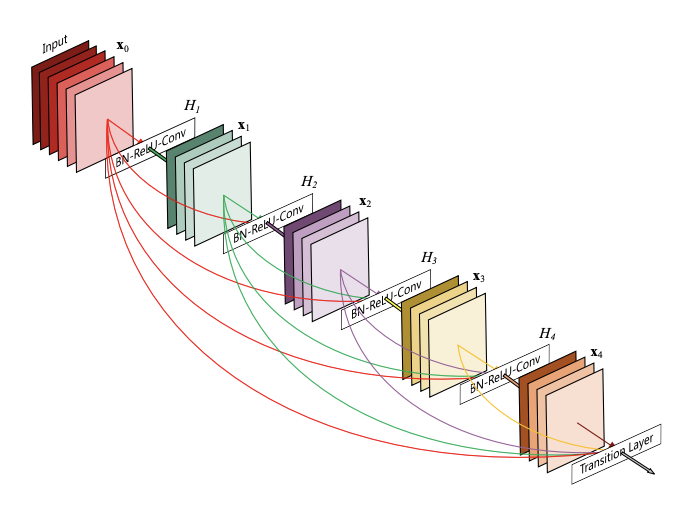
\includegraphics[width=.5\linewidth]{figures/models/denseblock}
	\caption[Densely Connected Block]{Densely Connected Block}
	\label{fig:denseblock}
\end{figure}

The densely connected layers are similarly to residual network grouped into resolution block called dense blocks, but for \gls{densenet} intermediate transition layers are added between dense block to downsample the feature size. 

\begin{figure}
	\centering
	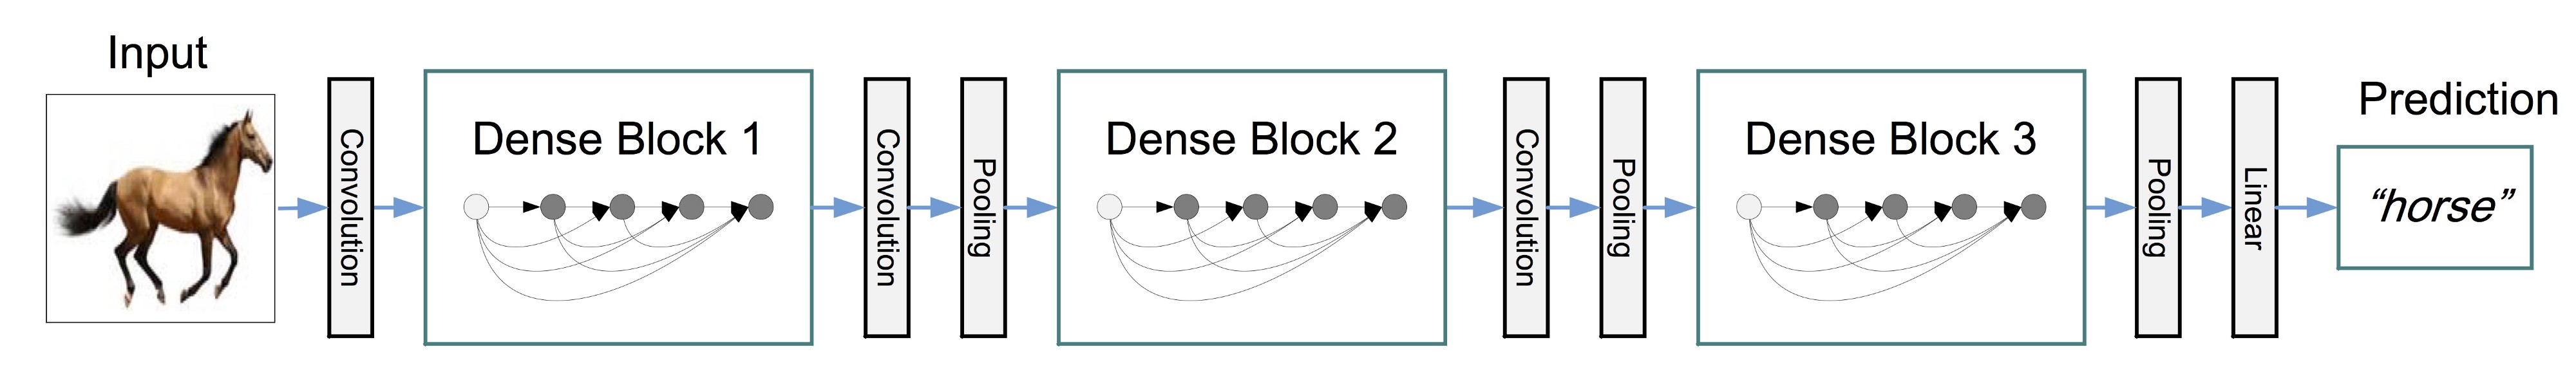
\includegraphics[width=\linewidth]{figures/models/densenet}
	\caption[Densely Connected Block]{Densely Connected Block}
	\label{fig:densenet}
\end{figure}

The collective knowledge from all preceding layers gives more diversified features compared to the correlated features of \gls{resnet}s. In \cite{huang_multi-scale_2017} the diversified features are shown to be more suited for early exiting,  as the information are better preserved using dense connection, hence even though information may have been collapsed to generate a short-term feature for the classifier. Thus placement of an intermediate classifier have less impact on the learned features for a later classifier. \gls{densenet} can be thinner as the number of channel can be fewer, thus more efficient compared to traditional and residual networks. Additionally densely connected blocks have a regularizing effect thus reducing overfitting the training data, hence perform better on smaller training sets. 

Table \ref{tbl:densenet121} describes the block and layers of the \gls{densenet} architecture. 

\begin{minipage}{\linewidth}
\begin{longtabu}{>{\bfseries}X|X[c]|X[2c]}
	\caption[\gls{densenet}-121 description]{\gls{densenet}-121 description. The table describes the blocks of \gls{densenet}-121. $k$ is the growth rate of the DenseBlock. A typical setting is $k=32$ yielding 256, 512 and 1024 output channels for denseblock(1-3) respectively. The transition layer downsamples the output channel by a factor of 2, thus the number of input channels for DenseBlock(2-4) becomes 128, 256 and 512 respectively.} \label{tbl:densenet121} \\
	\toprule
	\rowfont{\bfseries}
	Layers & Output size & Layer description \tabularnewline
	\hline
	\endfirsthead
	\multicolumn{3}{@{}l}{\textbf{\textcolor{black}{Table \ref{tbl:resnet50}:}} continued}\\
	\toprule
	\rowfont{\bfseries}
	Layers & Output size & Layer description \tabularnewline
	\hline
	\endhead % all the lines above this will be repeated on every page
	\hline
	\multicolumn{3}{@{}l}{continued \ldots}\\
	\endfoot
	\hline
	\endlastfoot
	Convolution & $112\times 112$& $7\times 7, \:\mathrm{stride}\: 2$ \tabularnewline \hline
	Pooling & $56\times 56$& $3\times 3, \:\mathrm{maxpool},\:  \mathrm{stride}\: 2$ \tabularnewline \hline
	\multirow{3}{*}{DenseBlock (1)} 	& \multirow{3}{*}{$56 \times 56$} & \multirow{3}{*}{
		$\begin{bmatrix}
		1 \times 1, k \\ 3 \times 3, k \\
		\end{bmatrix} \times 6$ }		\tabularnewline										
	& &  	\tabularnewline
	& & 	\tabularnewline
	\hline
	
	Transition  	& $56 \times 56$ & $1 \times 1\: \mathrm{conv}$ \tabularnewline \tabucline{2-3}							
	Layer (1) & $28\times 28$ & $2\times 2\: \mathrm{average\: pool,\: stride}\: 2$	\tabularnewline
	
	\hline
	
	\multirow{3}{*}{DenseBlock (2)} 	& \multirow{3}{*}{$28 \times 28$} & \multirow{3}{*}{
		$\begin{bmatrix}
		1 \times 1, k \\ 3 \times 3, k \\
		\end{bmatrix} \times 12$ }		\tabularnewline										
	& &  	\tabularnewline
	& & 	\tabularnewline
	\hline
	
	Transition  	& $28 \times 28$ & $1 \times 1\: \mathrm{conv}$ \tabularnewline \tabucline{2-3}							
	Layer (2) & $14\times 14$ & $2\times 2\: \mathrm{average\: pool,\: stride}\: 2$	\tabularnewline
	
	\hline
	
	\multirow{3}{*}{DenseBlock (3)} 	& \multirow{3}{*}{$14 \times 14$} & \multirow{3}{*}{
		$\begin{bmatrix}
		1 \times 1, k \\ 3 \times 3, k \\
		\end{bmatrix} \times 24$ }		\tabularnewline										
	& &  	\tabularnewline
	& & 	\tabularnewline
	\hline
	
	Transition  	& $14 \times 14$ & $1 \times 1\: \mathrm{conv}$ \tabularnewline \tabucline{2-3}							
	Layer (3) & $7\times 7$ & $2\times 2\: \mathrm{average\: pool,\: stride}\: 2$	\tabularnewline
	
	\hline
	
	\multirow{3}{*}{DenseBlock (4)} 	& \multirow{3}{*}{$7 \times 7$} & \multirow{3}{*}{
		$\begin{bmatrix}
		1 \times 1, k \\ 3 \times 3, k \\
		\end{bmatrix} \times 16$ }		\tabularnewline										
	& &  	\tabularnewline
	& & 	\tabularnewline
	\hline
	
	Classification  	& $1 \times 1$ & $7 \times 7\: \mathrm{global\: average\: pool}$ \tabularnewline \tabucline{2-3}							
	Layer &  \multicolumn2{c}{$\mathrm{Avg.\: Pool,\:} 1000d\: \mathrm{fc,\: Softmax}$} \tabularnewline
	\bottomrule
\end{longtabu}
\color{caption-color}{\textit{Source: \citetitle{huang_densely_2016}, by \citeauthor{huang_densely_2016} \cite{huang_densely_2016}, describes a full list of Densely Connected Networks (\gls{densenet}-121, \gls{densenet}-169, \gls{densenet}-201 and \gls{densenet}-264)}} \color{main-color}
\end{minipage}


In the same fashion as B-ResNet early exits have been placed to construct B-DenseNet. The exits are placed after a DenseBlock to obtain feature of sufficient quality and exiting as quickly as possible. If used in Edge-Device mode and the confidence was insufficient the transition layer after the DenseBlock is executed, before data is being preprocess for offloading.





\section{BranchyNet Training}

%\begin{figure}
%	\centering
%	\captionsetup[subfigure]{justification=centering}
%	\subfloat[Train loss\label{fig:B-resnet-miniimagenet10-train-loss}]{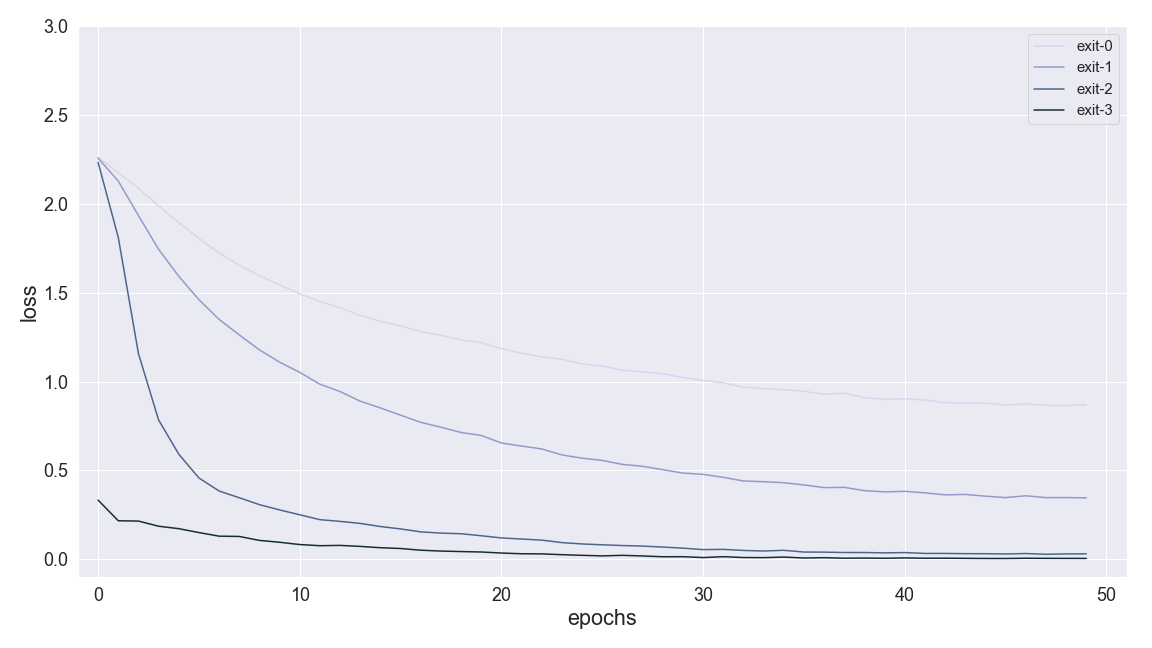
\includegraphics[width=.49\textwidth]{figures/bresnet_mini10/BResNet_train_loss_miniimagenet10.png}}
%	\subfloat[Test loss \label{fig:B-resnet-miniimagenet10-test-loss}]{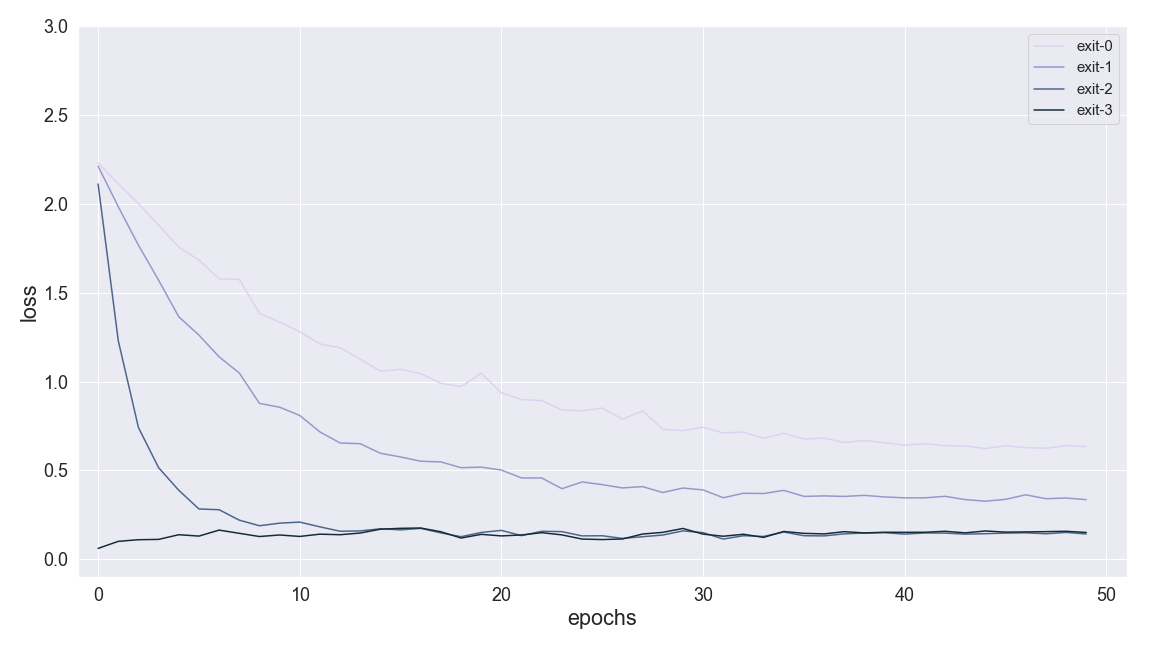
\includegraphics[width=.49\textwidth]{figures/bresnet_mini10/BResNet_test_loss_miniimagenet10.png}}
%	\hfill
%	\subfloat[Train accuracy\label{fig:B-resnet-miniimagenet10-train-acc}]{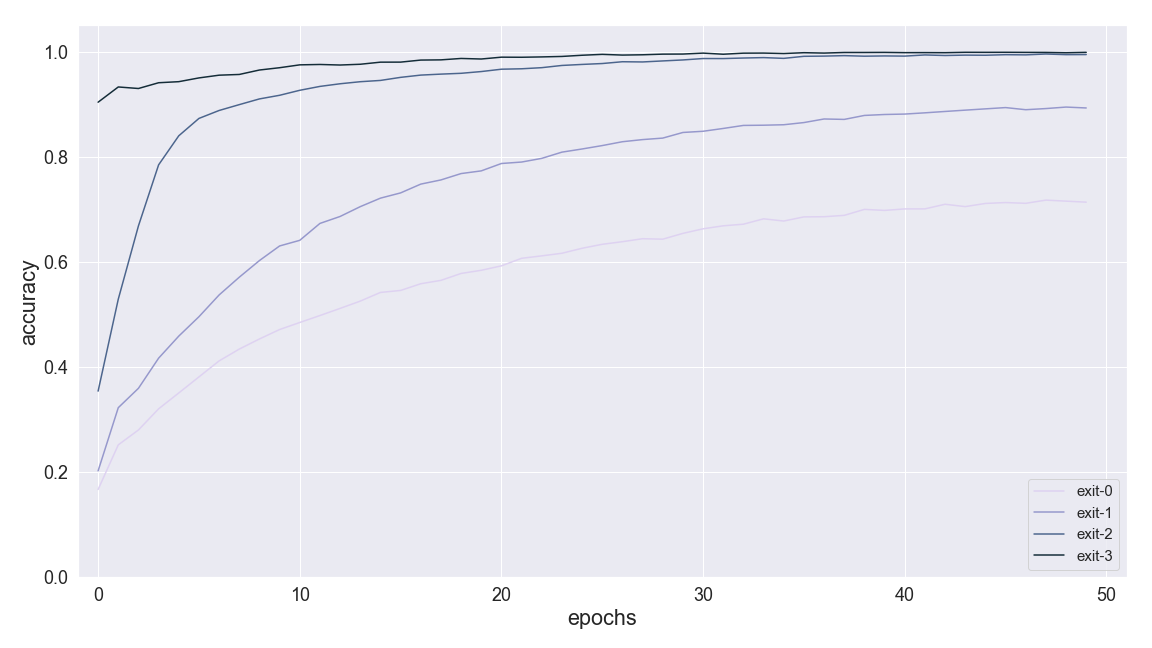
\includegraphics[width=.49\textwidth]{figures/bresnet_mini10/BResNet_train_acc_miniimagenet10.png}}
%	\subfloat[Test accuracy\label{fig:B-resnet-miniimagenet10-test-acc}]{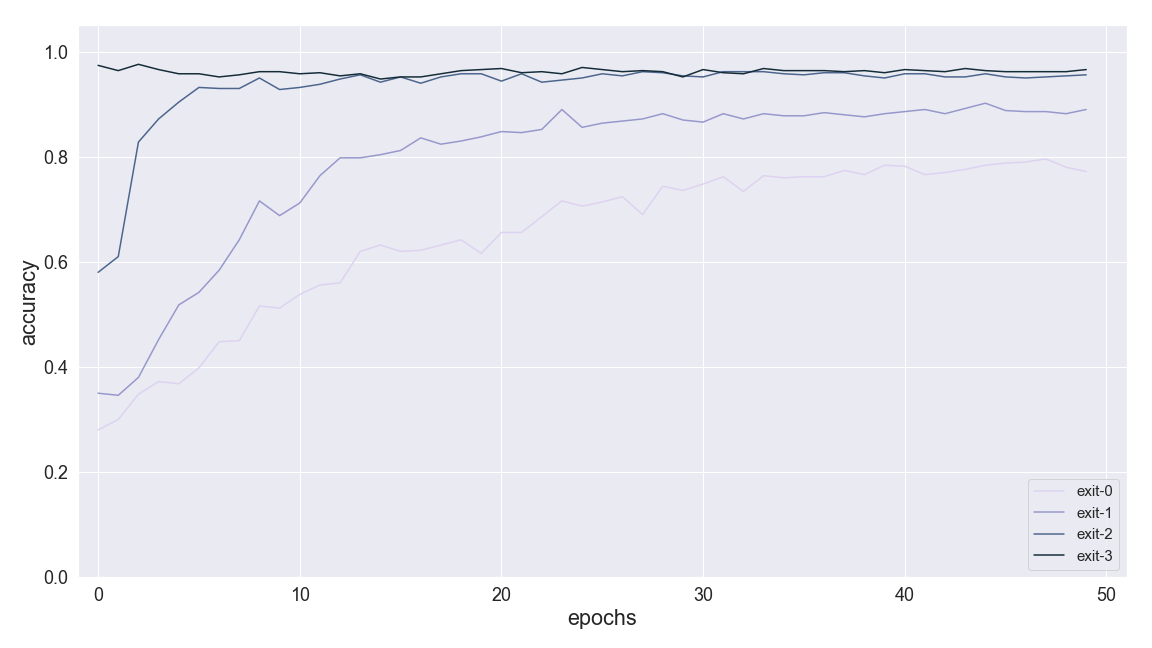
\includegraphics[width=.49\textwidth]{figures/bresnet_mini10/BResNet_test_acc_miniimagenet10.png}}
%	\caption[B-ResNet MiniImageNet10 Training summary]{Training summary shows the progression of model attributes over times of epochs, \protect\subref{fig:B-resnet-miniimagenet10-train-loss} train loss, \protect\subref{fig:B-resnet-miniimagenet10-test-loss} test loss, \protect\subref{fig:B-resnet-miniimagenet10-train-acc} train accuracy, \protect\subref{fig:B-resnet-miniimagenet10-test-acc}, test accuracy.}
%	\label{fig:B-resnet-miniimagenet-10}
%\end{figure}

Training B-\gls{resnet} and B-\gls{densenet} shows the importance of the densely connected layers for an early exiting model. The early exits of B-\gls{densenet} have a higher accuracy compared to B-\gls{resnet}, however B-\gls{resnet} last two exits are more accurate, see figure \ref{fig:b-net-miniimagenet-100}. 

\begin{figure}
	\centering
	\captionsetup[subfigure]{justification=centering}
	\subfloat[B-Resnet\label{fig:B-resnet-miniimagenet100}]{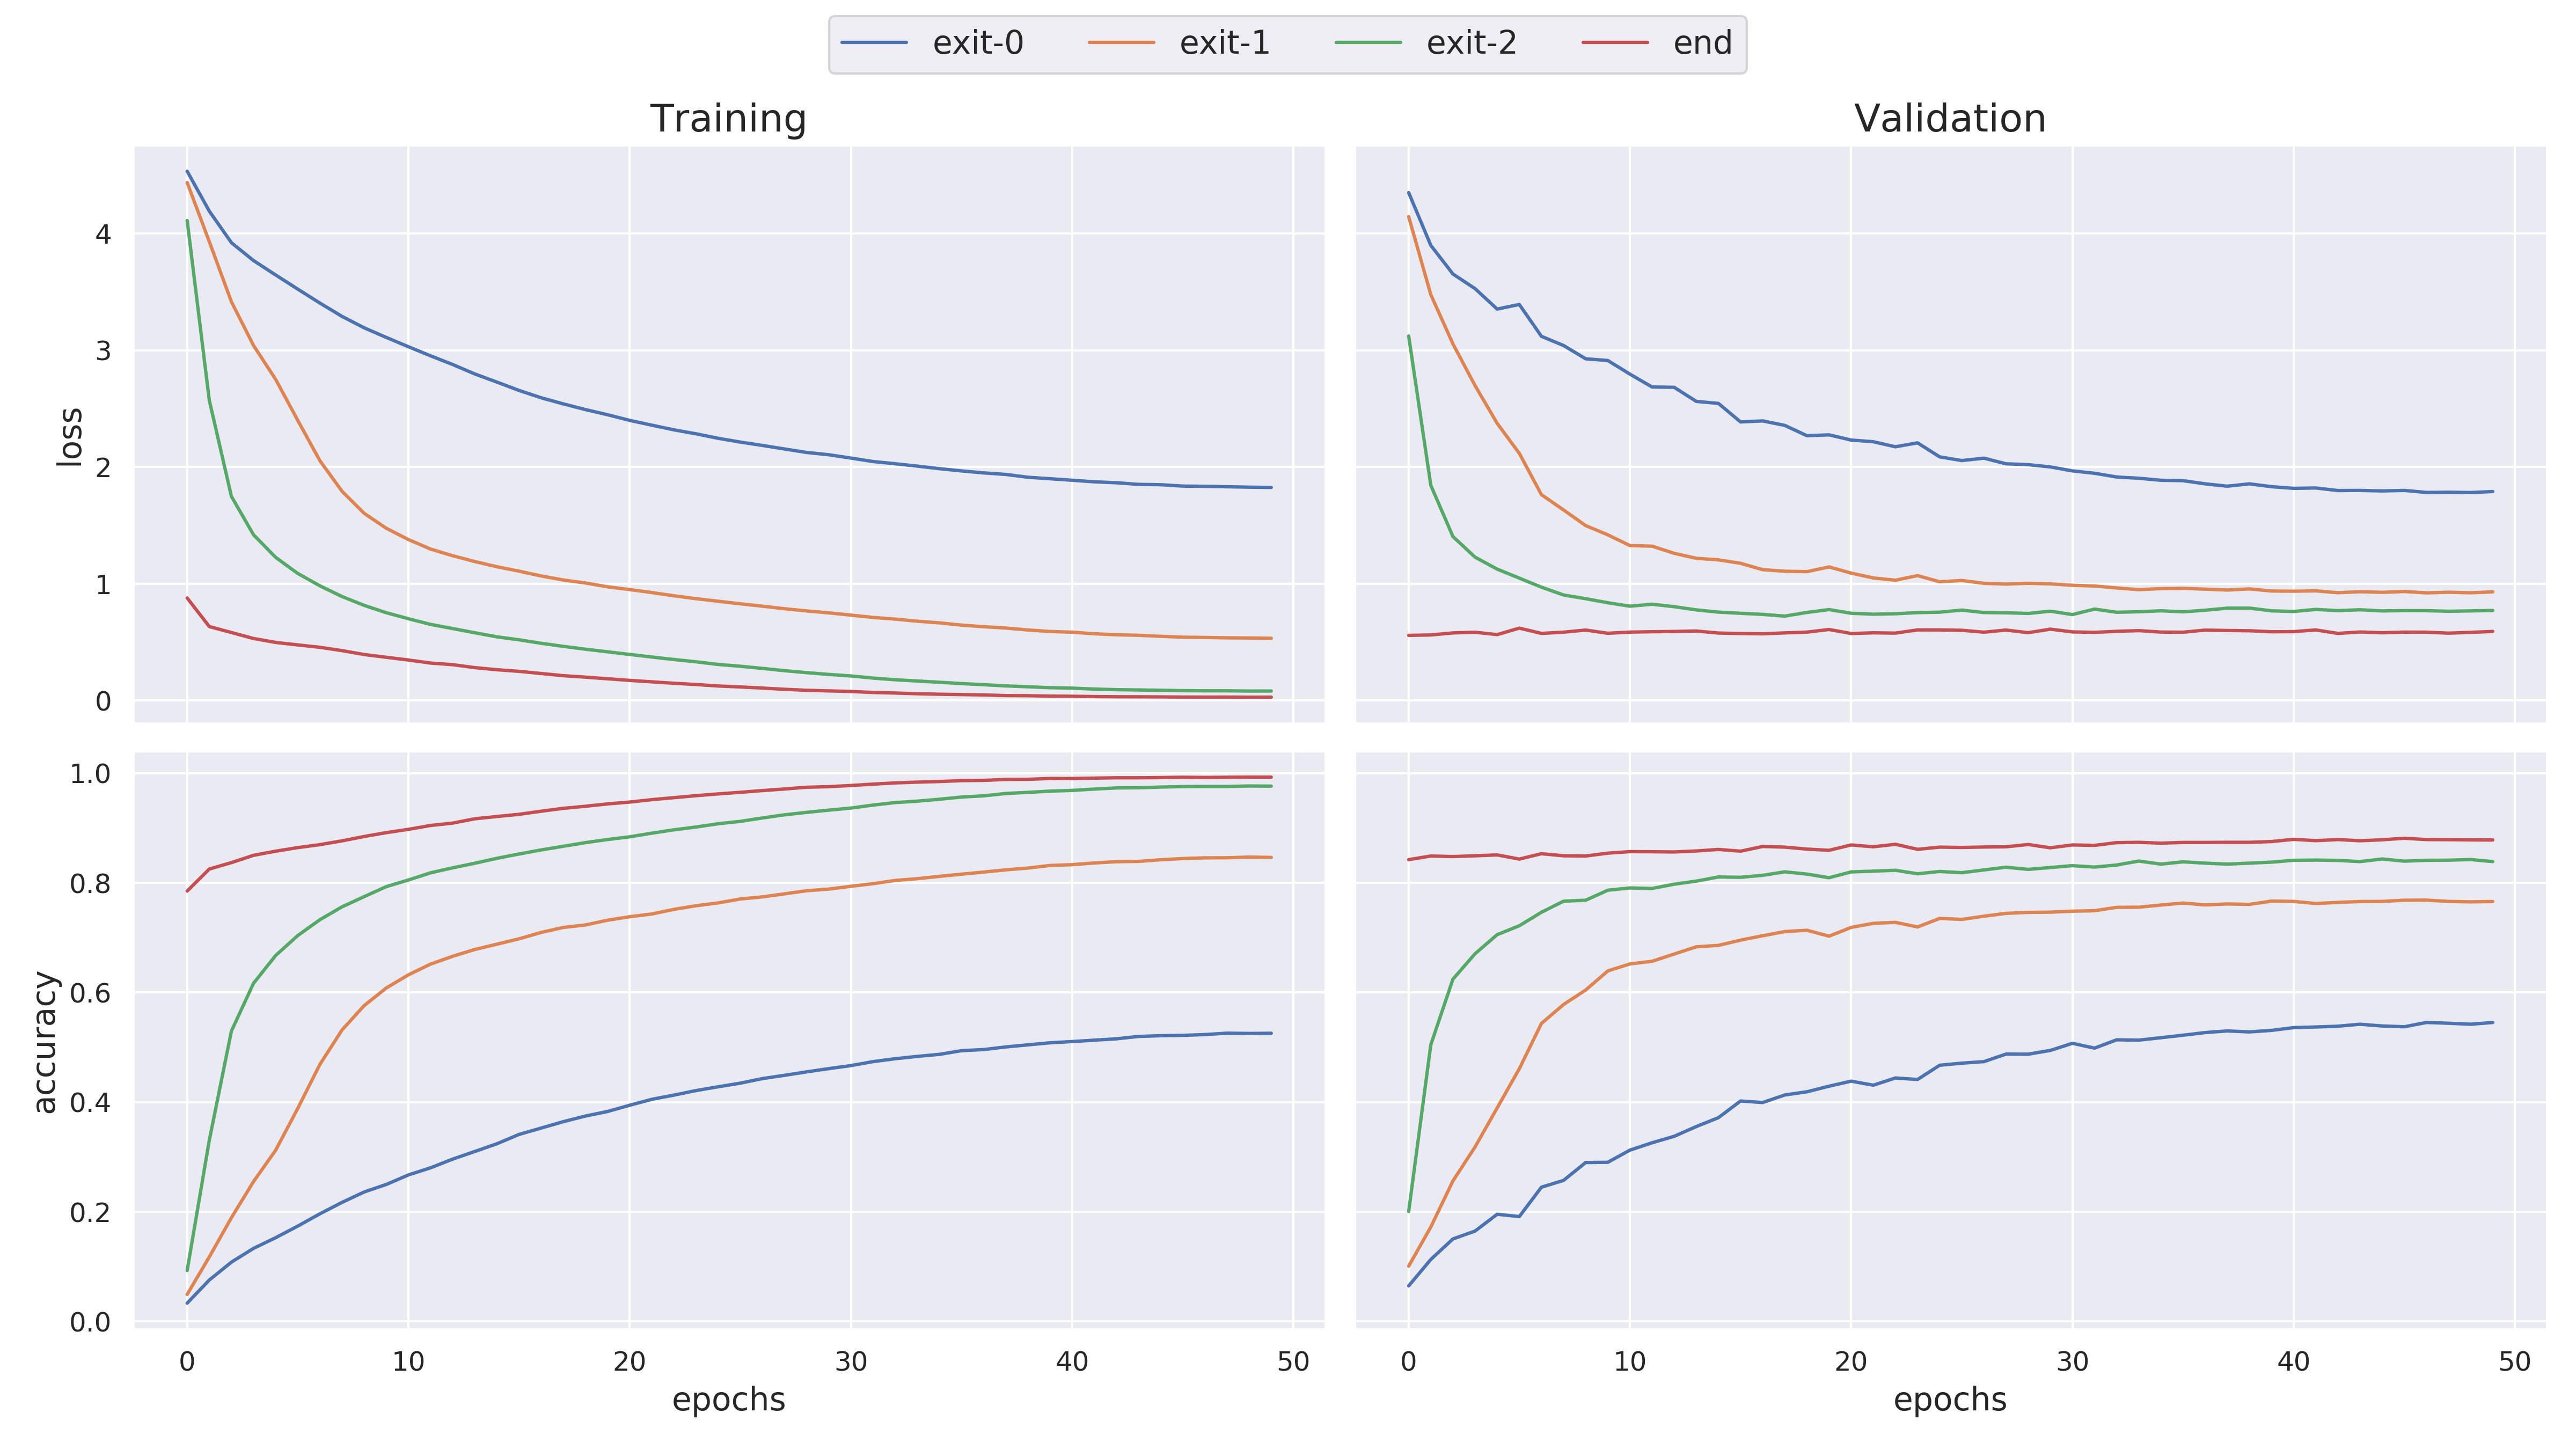
\includegraphics[width=\linewidth]{figures/training_plots/resnet_miniimagenet100}}
\end{figure}

The two last exits of \gls{resnet} are almost equally accurate. The resolution block of exit-2 are very deep, and the features becomes optimized for this classifier, hence not much gain in accuracy is obtained by running the early exit model all the way to the end. \gls{densenet} on the other hand always have an accuracy gain by continuing the inference process.    

\begin{figure}
	%\ContinuedFloat
	\captionsetup[subfigure]{justification=centering}
	\subfloat[B-DenseNet\label{fig:B-densenet-miniimagenet100}]{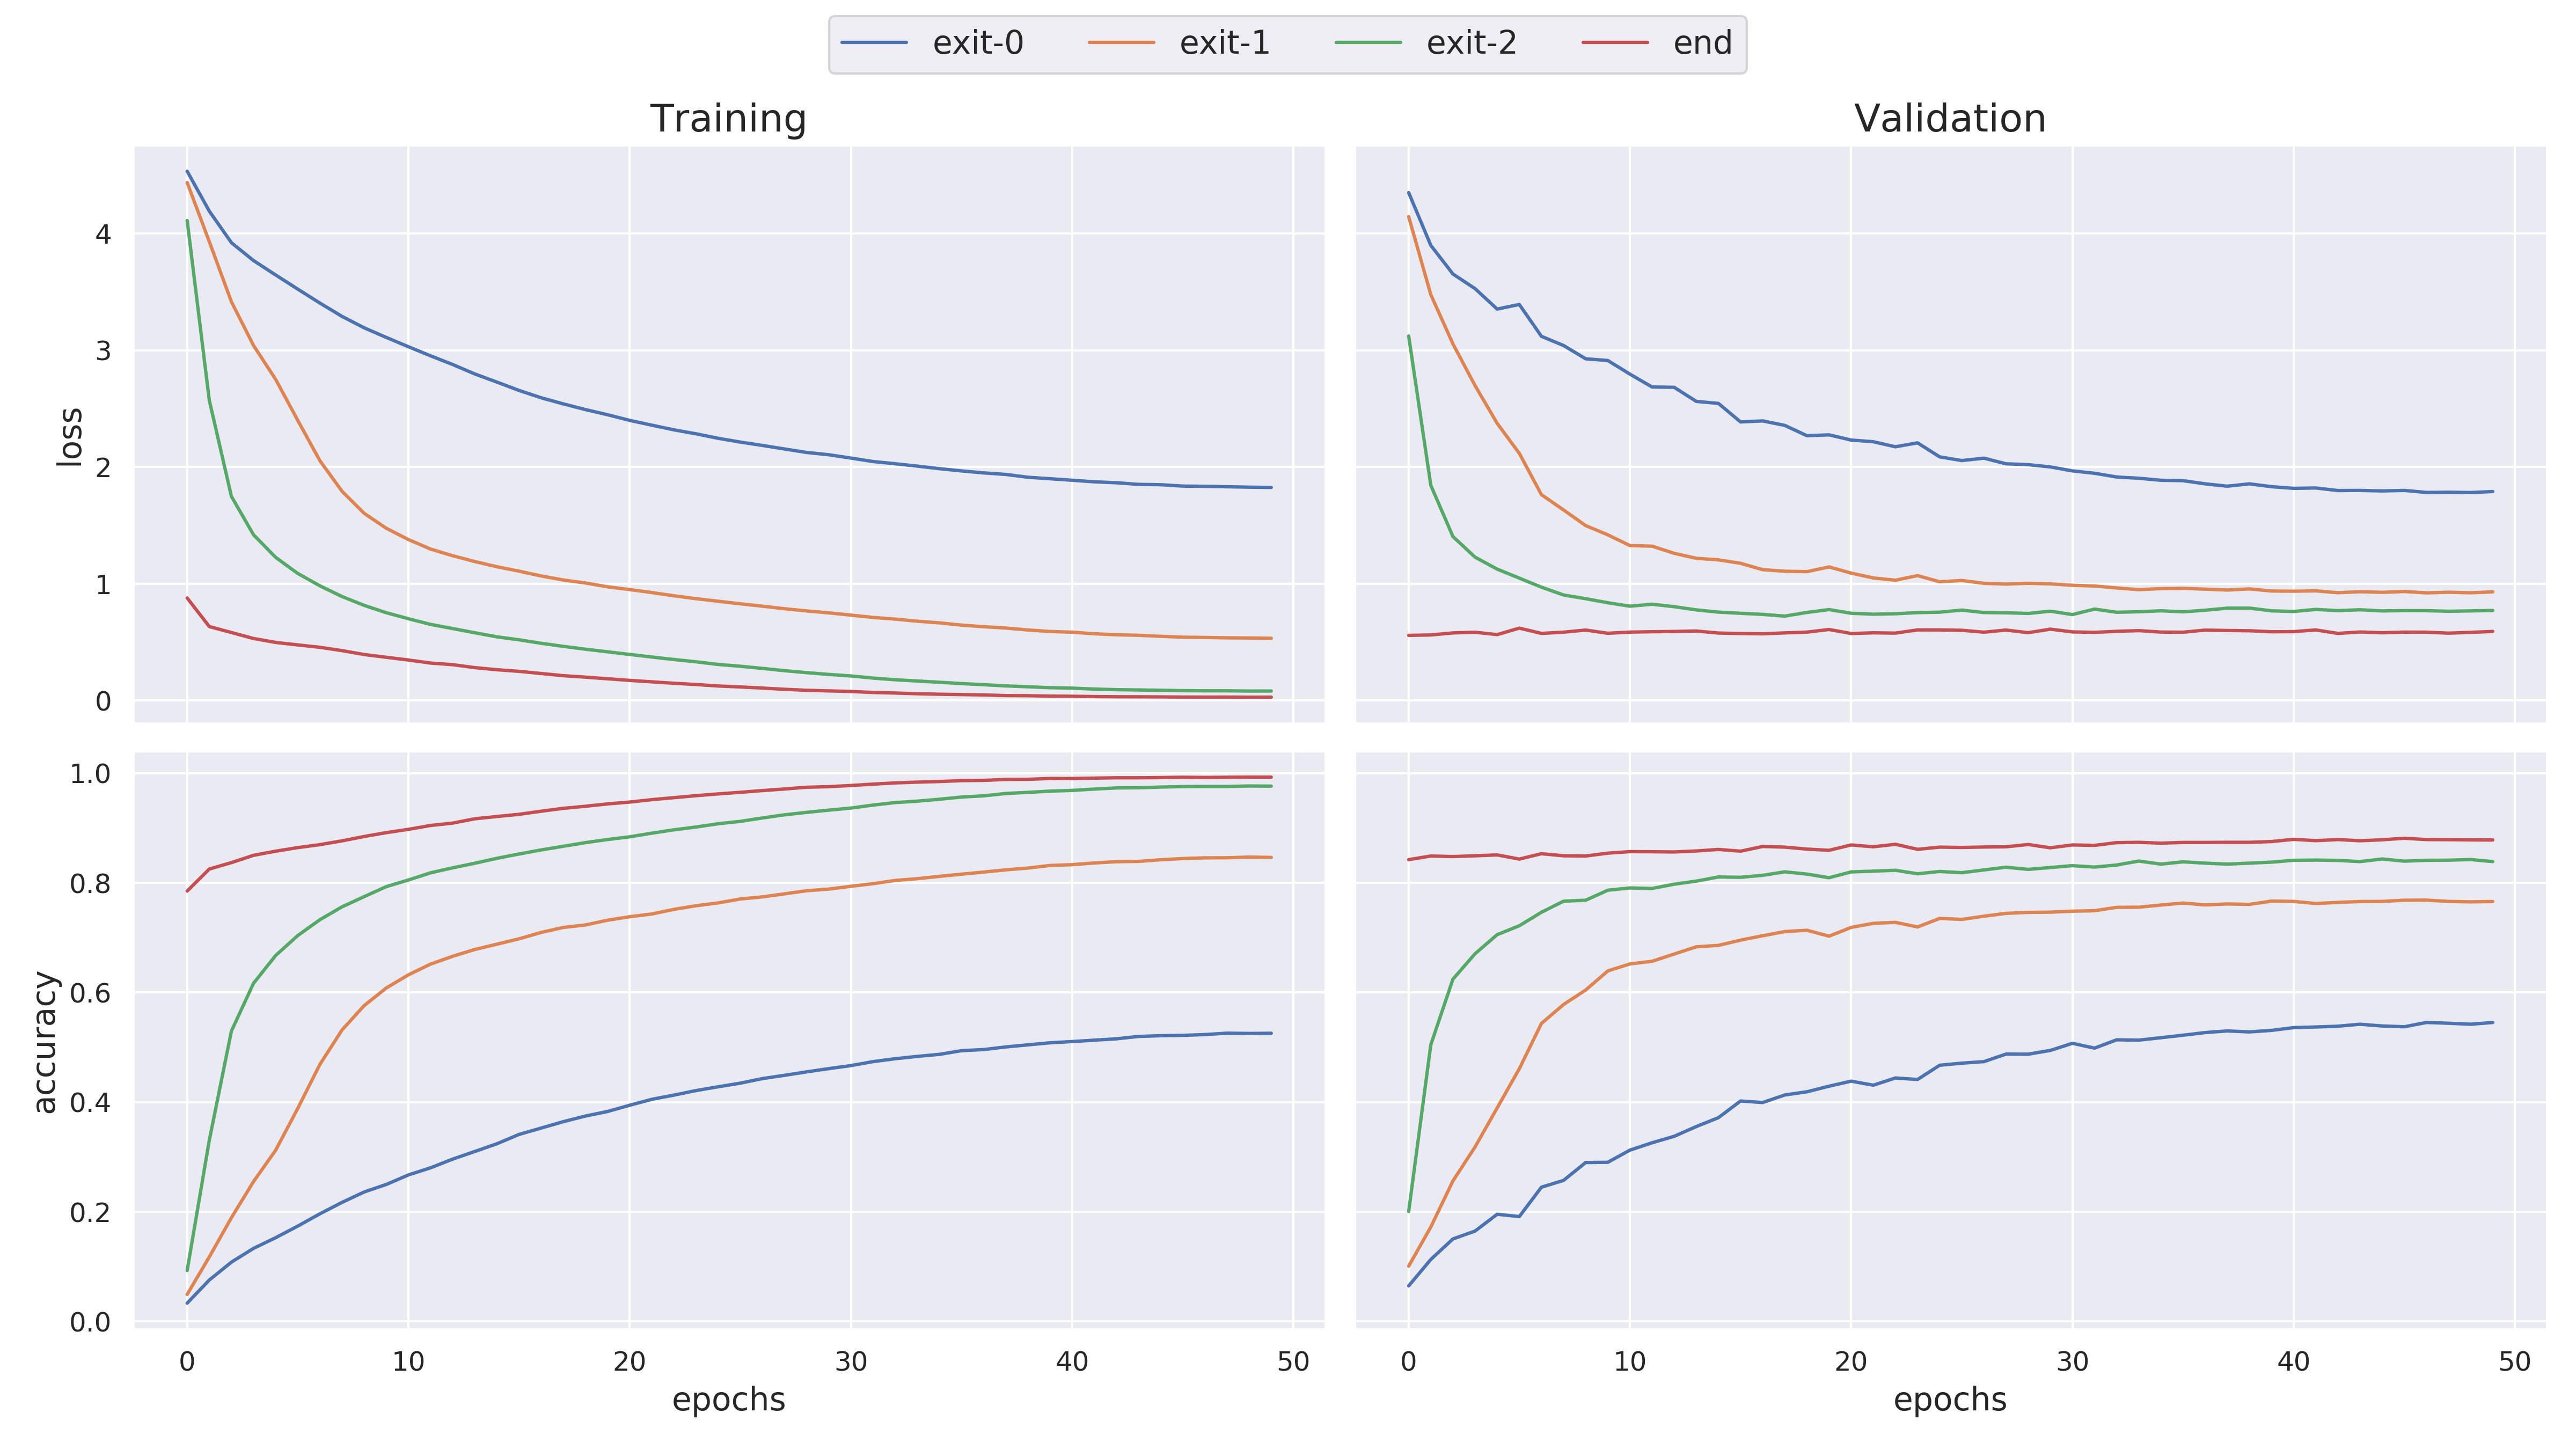
\includegraphics[width=\linewidth]{figures/training_plots/densenet_miniimagenet100}}
\end{figure}

\begin{figure}
	%\ContinuedFloat
	\captionsetup[subfigure]{justification=centering}
	\subfloat[MSDNet\label{fig:msdnet-miniimagenet100}]{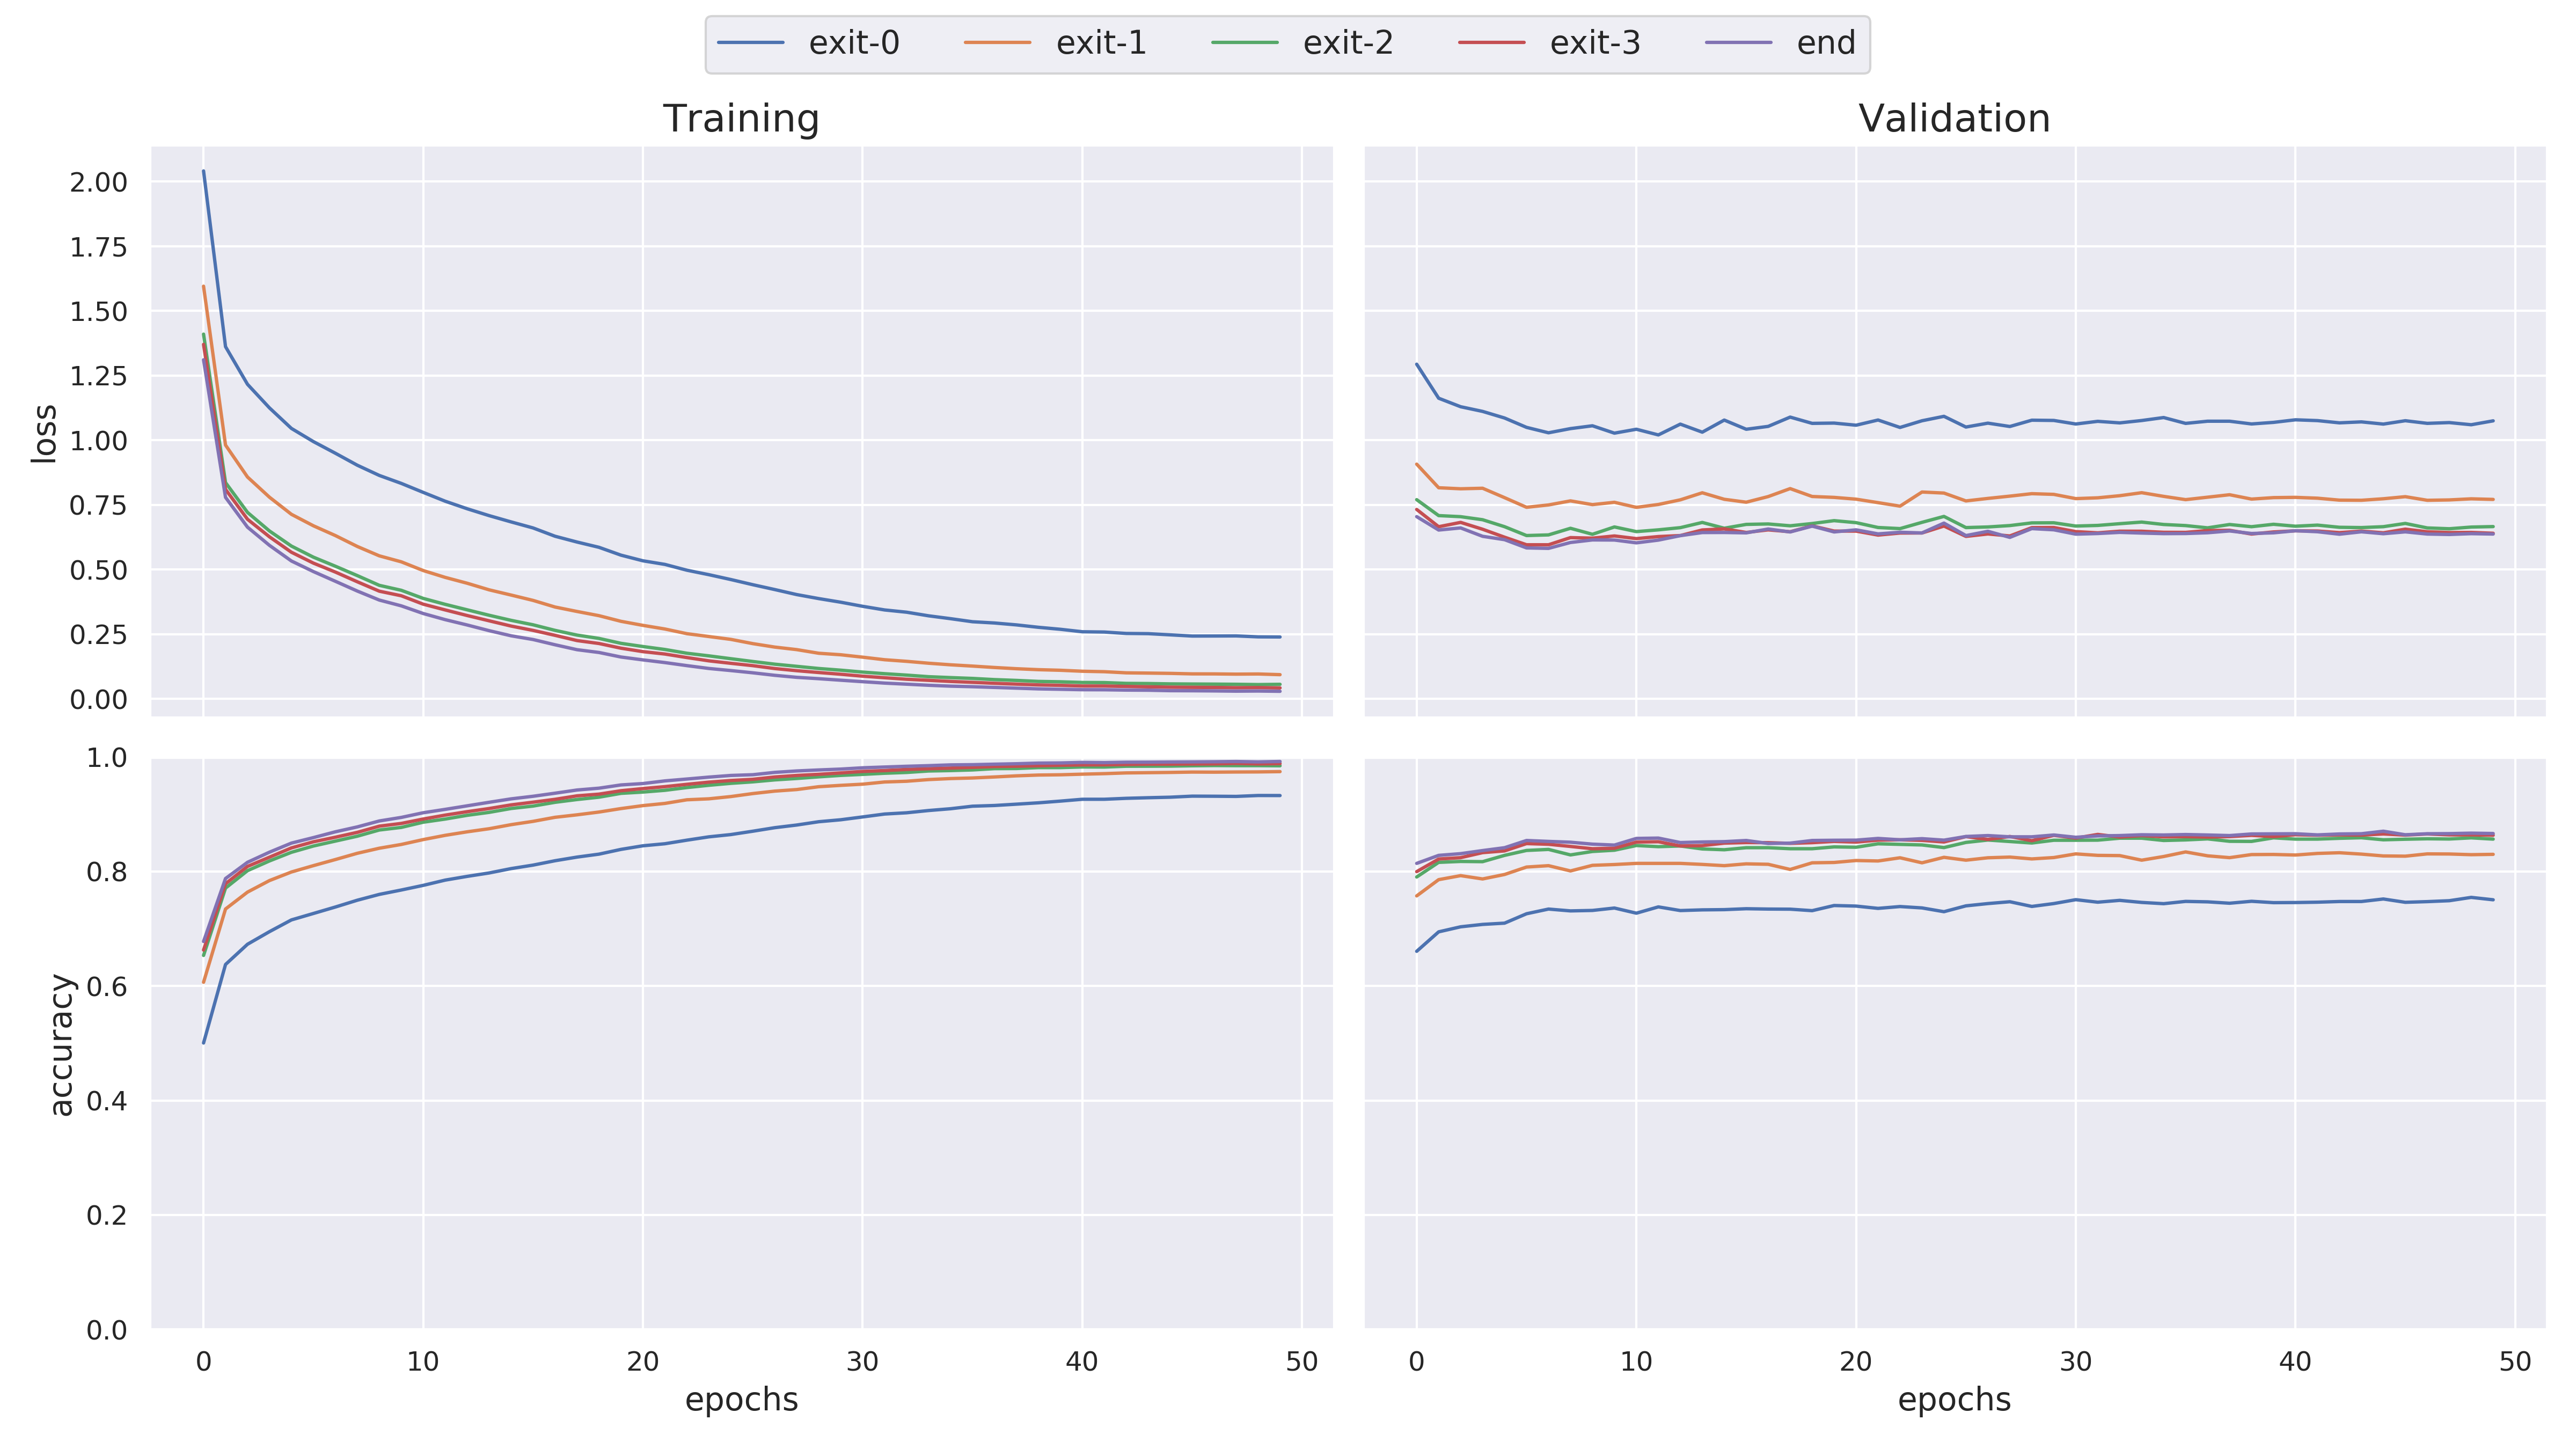
\includegraphics[width=\linewidth]{figures/training_plots/msd_miniimagenet100}}
	\caption[Training progress of BrancyNets]{Training progress for \protect\subref{fig:B-resnet-miniimagenet100} B-ResNet, \protect\subref{fig:B-densenet-miniimagenet100} B-DenseNet and \protect\subref{fig:msdnet-miniimagenet100} MSDNet} 
	\label{fig:b-net-miniimagenet-100}
\end{figure}


\section{Inference Testing}

In this test all validation samples are inferred to all three models. Each branch classifies the samples, but does not perform exit but continues the inference process. Figure \ref{fig:exit-accuracy} show the accuracy of each exit.  

\begin{figure}
	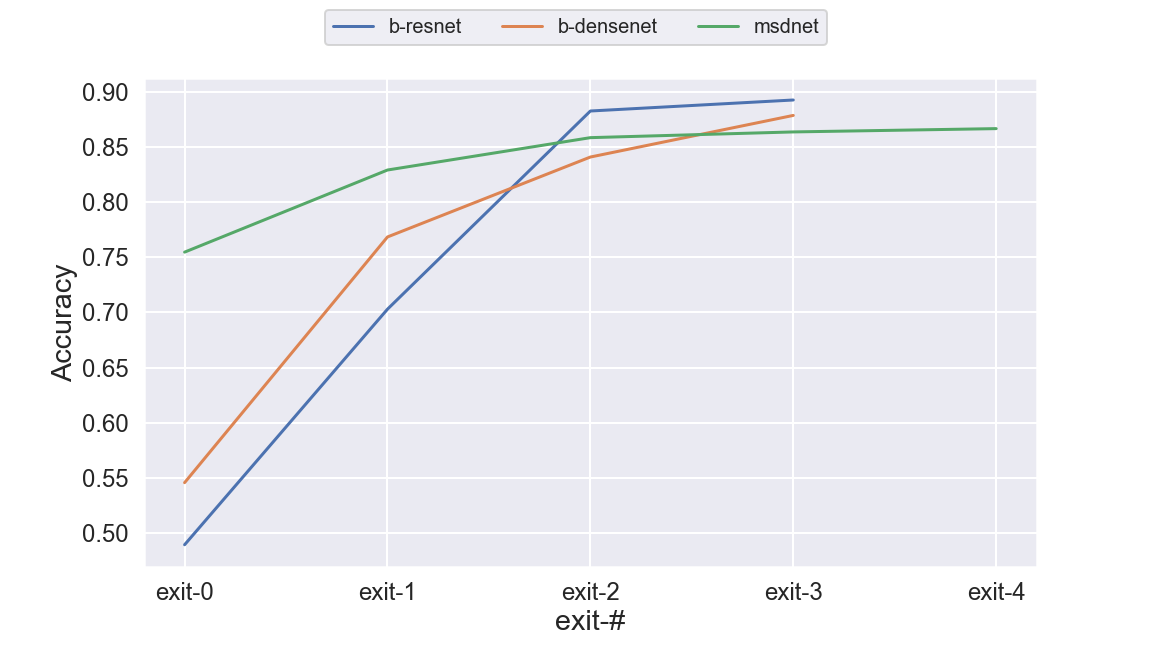
\includegraphics[width=\linewidth]{figures/inference_plots/exit_acc}
	\caption[Model Inference Accuracy]{Model Inference Accuracy}
	\label{fig:exit-accuracy}
\end{figure}

As expected the models become more accurate as we go deeper in the network. The features deep within the network have more discriminative characteristics. As stated in \cite{huang_multi-scale_2017} the densely connected features are important factors for obtaining intermediate classifiers with decent accuracy. The B-\gls{densenet} and \gls{msdnet} have as expected more accurate early classifiers, however the end-exit of B-\gls{resnet} achieves superior accuracy compared to the other models.

Still about half the samples can be accurately classified at the very first exit, which justifies the assumption for \gls{branchynet} and we can expectedly save time but let samples exit prematurely, see figure \ref{fig:exit-time}

\begin{figure}
	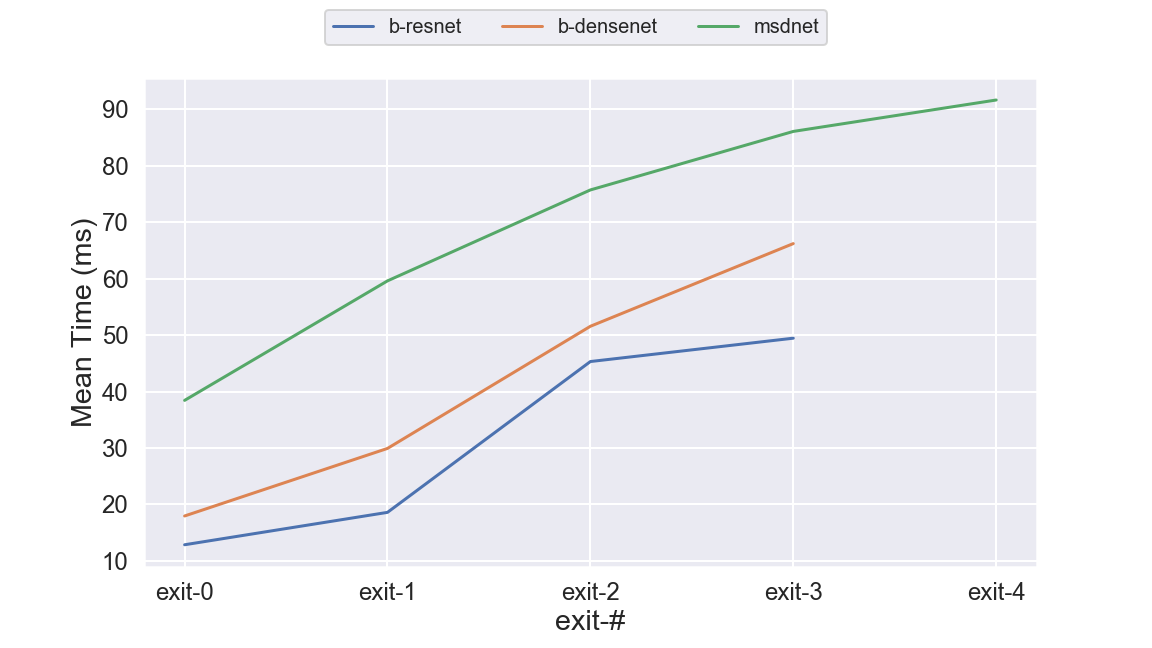
\includegraphics[width=\linewidth]{figures/inference_plots/exit_time}
	\caption[Model Inference Accuracy]{Model Inference Time}
	\label{fig:exit-time}
\end{figure}

Figure \ref{fig:exit-time} shows the average inference time for a classification at the corresponding exit. If the model decides to exit earlier in the network, the figure shows the time savings achievable. The inference time is hardware dependent and a full model comparison cannot be made solely by this test, later tests compares the inference time of the models on different platforms, however the trend seems to be, that B-\gls{resnet} is the fastest, followed by B-\gls{densenet} an lastly \gls{msdnet}. Table \ref{tbl:early-exit} shows the accuracy and mean time in tabular form.

\begin{longtabu}{>{\bfseries}X|X|X}
	\caption[Early exit models' last exit accuracy]{Early exit models' last exit accuracy}\label{tbl:early-exit} \\
	\toprule
	\rowfont{\bfseries}
	Model & Accuracy & Mean Time (ms) \tabularnewline
	\hline
	\endfirsthead
	\multicolumn{3}{@{}l}{\textbf{\textcolor{black}{Table \ref{tbl:early-exit}:}} continued}\\
	\toprule
	\rowfont{\bfseries}
	Model & Accuracy & Mean Time (ms) \tabularnewline
	\hline
	\endhead % all the lines above this will be repeated on every page
	\hline
	\multicolumn{3}{@{}l}{continued \ldots}\\
	\endfoot
	\hline
	\endlastfoot
	B-ResNet & \tabularnewline
	\hspace{3mm} Exit-0 & 0.489 & 12.87 \tabularnewline
	\hspace{3mm} Exit-1 & 0.703 & 18.61 \tabularnewline
	\hspace{3mm} Exit-2 & 0.883 & 45.31 \tabularnewline
	\hspace{3mm} Exit-3 & 0.893 & 49.45 \tabularnewline
	\hline
	B-DenseNet &  \tabularnewline
	\hspace{3mm} Exit-0 & 0.545 & 17.96 \tabularnewline
	\hspace{3mm} Exit-1 & 0.769 & 29.93 \tabularnewline
	\hspace{3mm} Exit-2 & 0.841 & 51.56 \tabularnewline
	\hspace{3mm} Exit-3 & 0.879 & 66.20 \tabularnewline
	\hline
	MSDNet & \tabularnewline
	\hspace{3mm} Exit-0 & 0.755 & 38.43 \tabularnewline
	\hspace{3mm} Exit-1 & 0.829 & 59.60 \tabularnewline
	\hspace{3mm} Exit-2 & 0.859 & 75.70 \tabularnewline
	\hspace{3mm} Exit-3 & 0.864 & 86.06 \tabularnewline
	\hspace{3mm} Exit-4 & 0.867 & 91.63 \tabularnewline
	\bottomrule
\end{longtabu}

The challenge is to known when to let samples exit, which can either be done at random or using the output from the softmax function, which can be interpreted as a confidence metric for the prediction. In the next test, we evaluate the two mentioned confidence scores as a threshold for exiting. 


%\paragraph{Pascal VOC}
%
%\begin{figure}
%	\centering
%	\captionsetup[subfigure]{justification=centering}
%	\subfloat[Train loss\label{fig:B-resnet-voc-train-loss}]{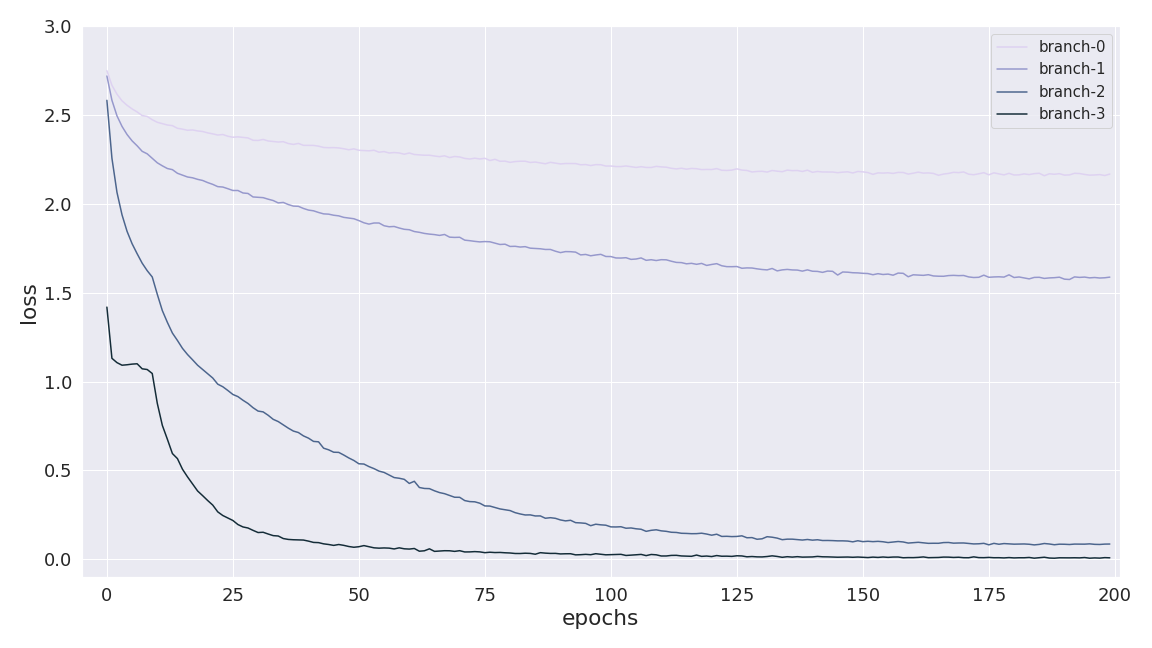
\includegraphics[width=.49\textwidth]{figures/BResNetVOC/BResNet_train_loss_VOC.png}}
%	\subfloat[Test loss \label{fig:B-resnet-voc-test-loss}]{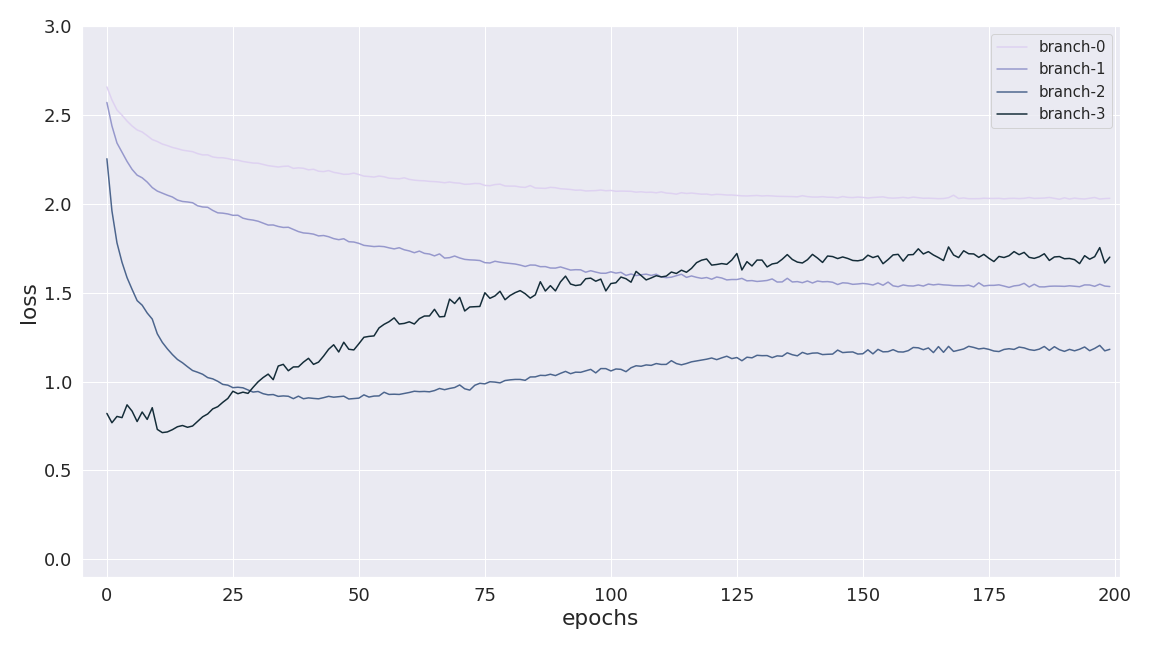
\includegraphics[width=.49\textwidth]{figures/BResNetVOC/BResNet_test_loss_VOC.png}}
%	\hfill
%	\subfloat[Train accuracy\label{fig:B-resnet-voc-train-acc}]{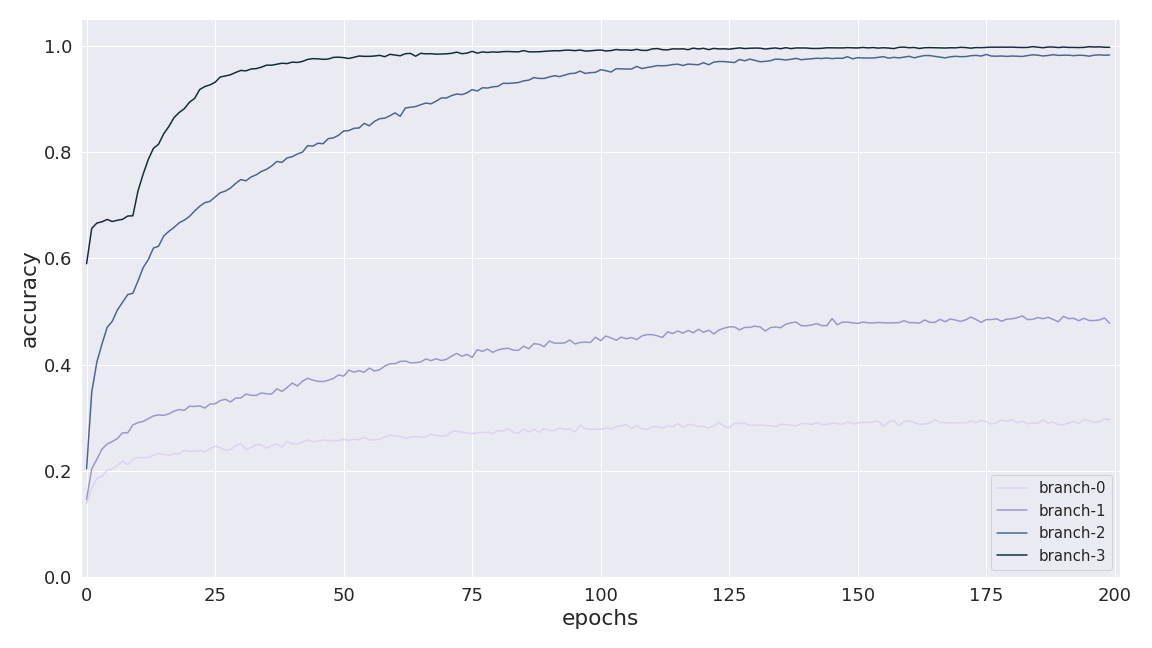
\includegraphics[width=.49\textwidth]{figures/BResNetVOC/BResNet_train_acc_VOC.png}}
%	\subfloat[Test accuracy\label{fig:B-resnet-voc-test-acc}]{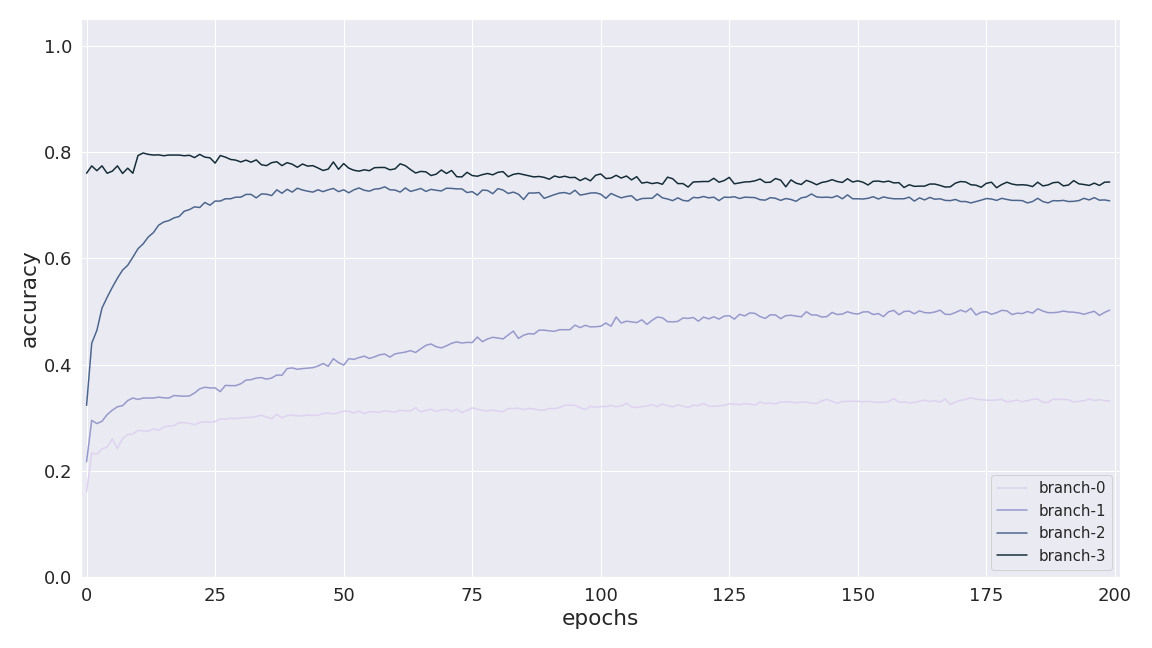
\includegraphics[width=.49\textwidth]{figures/BResNetVOC/BResNet_test_acc_VOC.png}}
%	\caption[B-ResNet VOC Training summary]{Training summary shows the progression of model attributes over times of epochs, \protect\subref{fig:B-resnet-voc-train-loss} train loss, \protect\subref{fig:B-resnet-voc-test-loss} test loss, \protect\subref{fig:B-resnet-voc-train-acc} train accuracy, \protect\subref{fig:B-resnet-voc-test-acc}, test accuracy.}
%\end{figure}
%
%Visualizing the training progression, clearly indicates that model overfitting to the training data. When a model overfits it suffers to generalize the true underlying distribution of the data. This can be caused by insufficient number of training samples or too complex a model. Since the model has shown promising results in image classification task previously, we can conclude, that the dataset is too sparse.
%
%Even though the model fails to generalize, the experiment still produce interesting results. Given an early exiting model as B-ResNet 50\% of the test samples can be correctly classified using only half of the \gls{dnn}.


\section{Threshold Analysis}

In this experiment the MiniImageNet100 validation set have been used to evaluate the two threshold metrics; \emph{Confidence Threshold} and \emph{Score-Margin Threshold}. \Cref{fig:resnet_confidence,fig:resnet_score-margin,fig:densenet_confidence,fig:densenet_score-margin,fig:msdnet_confidence,fig:msdnet_score-margin} compares the performance of each exit on all samples. The figures show for each of the three networks under test a plot of the two thresholds for all exit for the model. It shows the frequency of exited samples, that have been correctly classified ({\color{sns-green}green}) and incorrectly classified ({\color{sns-red}red}). As well as, samples that could not be classified with proper confidence given the threshold metric, hence not exited at the exit ({\color{sns-blue}blue}). Along with a plot of the change in accuracy for the exit as the confidence grows ({\color{sns-orange}orange}).  

\newcounter{imagenumber}
\begin{minipage}{\textwidth}
\begin{figure}
	\centering
	\paragraph{B-ResNet}
	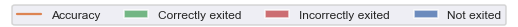
\includegraphics[width=\linewidth]{figures/threshold_plots/threshold_analysis_legend}
\end{figure}

\begin{minipage}{0.5\textwidth}
	\begin{figure}
		\captionsetup[subfloat]{farskip=1pt,captionskip=1pt, justification=centering}
		\centering
		\forloop{imagenumber}{0}{\value{imagenumber} < 4}{
			
			\subfloat[Exit-\arabic{imagenumber}\label{fig:confidence_resnet_exit_\arabic{imagenumber}}]{\includegraphics[width=.9\linewidth]{figures/threshold_plots/threshold_analysis_b-resnet_confidence_\arabic{imagenumber}}}
			\hfill
		}
		\caption[ResNet Confidence Threshold]{Confidence Threshold}
		\label{fig:resnet_confidence}
	\end{figure}
\end{minipage}
\begin{minipage}{0.5\textwidth}
	\begin{figure}
		\captionsetup[subfloat]{farskip=1pt,captionskip=1pt, justification=centering}
		\centering
		\forloop{imagenumber}{0}{\value{imagenumber} < 4}{
			
			\subfloat[Exit-\arabic{imagenumber}\label{fig:score-margin_resnet_exit_\arabic{imagenumber}}]{\includegraphics[width=.9\linewidth]{figures/threshold_plots/threshold_analysis_b-resnet_score-margin_\arabic{imagenumber}}}
			\hfill
		}
		\caption[ResNet Score-margin Threshold]{Score-margin Threshold}
		\label{fig:resnet_score-margin}
	\end{figure}
\end{minipage}
\end{minipage}

\begin{minipage}{\textwidth}
	\begin{figure}
		\centering
		\paragraph{B-DenseNet}
	\end{figure}
	\begin{minipage}{0.5\textwidth}
		\begin{figure}
			\captionsetup[subfloat]{farskip=1pt,captionskip=1pt, justification=centering}
			\centering
			\forloop{imagenumber}{0}{\value{imagenumber} < 4}{
				
				\subfloat[Exit-\arabic{imagenumber}\label{fig:confidence_dense_exit_\arabic{imagenumber}}]{\includegraphics[width=.9\linewidth]{figures/threshold_plots/threshold_analysis_b-densenet_confidence_\arabic{imagenumber}}}
				\hfill
			}
			\caption[DenseNet Confidence Threshold]{Confidence Threshold}
			\label{fig:densenet_confidence}
		\end{figure}
	\end{minipage}
	\begin{minipage}{0.5\textwidth}
		\begin{figure}
			\captionsetup[subfloat]{farskip=1pt,captionskip=1pt, justification=centering}
			\centering
			\forloop{imagenumber}{0}{\value{imagenumber} < 4}{
				
				\subfloat[Exit-\arabic{imagenumber}\label{fig:score-dense_resnet_exit_\arabic{imagenumber}}]{\includegraphics[width=.9\linewidth]{figures/threshold_plots/threshold_analysis_b-densenet_score-margin_\arabic{imagenumber}}}
				\hfill
			}
			\caption[DenseNet Score-margin Threshold]{Score-margin Threshold}
			\label{fig:densenet_score-margin}
		\end{figure}
	\end{minipage}
\end{minipage}

\noindent\makebox[\textwidth][c]{\begin{minipage}{0.9\textwidth}
	\begingroup
	\leftskip=0cm plus 0.5fil \rightskip=0cm plus -0.5fil
	\parfillskip=0cm plus 1fil
	\paragraph{MSDNet}\par
	\endgroup
	
	\begin{minipage}{0.5\textwidth}
		\begin{figure}
			\captionsetup[subfloat]{farskip=0pt,captionskip=0pt, justification=centering}
			\centering
			\forloop{imagenumber}{0}{\value{imagenumber} < 5}{
				
				\subfloat[Exit-\arabic{imagenumber}\label{fig:confidence_msd_exit_\arabic{imagenumber}}]{\includegraphics[width=.9\linewidth]{figures/threshold_plots/threshold_analysis_msdnet_confidence_\arabic{imagenumber}}}
				\hfill
			}
			\caption[MSDNet Confidence Threshold]{Confidence Threshold}
			\label{fig:msdnet_confidence}
		\end{figure}
	\end{minipage}
	\begin{minipage}{0.5\textwidth}
		\begin{figure}
			\captionsetup[subfloat]{farskip=1pt,captionskip=1pt, justification=centering}
			\centering
			\forloop{imagenumber}{0}{\value{imagenumber} < 5}{
				
				\subfloat[Exit-\arabic{imagenumber}\label{fig:score-msdnet_exit_\arabic{imagenumber}}]{\includegraphics[width=.9\linewidth]{figures/threshold_plots/threshold_analysis_msdnet_score-margin_\arabic{imagenumber}}}
				\hfill
			}
			\caption[MSDNet Score-margin Threshold]{Score-margin Threshold}
			\label{fig:msdnet_score-margin}
		\end{figure}
	\end{minipage}
\end{minipage}}

The aim is to find the metric, that reduces the amount of incorrectly exited samples ({\color{sns-red}red}). Whenever samples are exited incorrectly, the overall accuracy of the models are reduced, if it could have been correctly classifed at later exit. The growing frequency of correctly exited samples ({\color{sns-green}green}) at later exits shows exactly this. As the threshold requirements are raised, it results in a higher accuracy for the exit, as the ratio between correctly exited and incorrectly exited grows. Even though all samples will be classified at the last exit, hence no sample is in fact exited at this last exit, still it shows the frequency of samples, that could not reach a confident score for the last exit. This means the accuracy for the last exit is not entirely correct.  Table \ref{tbl:early-exit} shows the accuracy of the exit, when all samples are exited at the exit. 

Generally \emph{score-margin} has more desirable traits, as less samples are incorrectly exited (red), only at the expense of a few additional samples not exited ({\color{sns-blue}blue}). The results matches \cite{park_big/little_2015}, which show a stronger correlation to actually being able to correctly predict samples given the \emph{score-margin threshold}. Henceforth the \emph{score-margin threshold} are used.

The former test is conducted b stamping all samples whether it could have been exited at the exited and if would have been correct or not. The test does not take into account if samples have been exited, then not reaching a later exit, if a exit is very confident yet incorrect. In the next test, this is accommodated for.

\begin{figure}
	\centering
	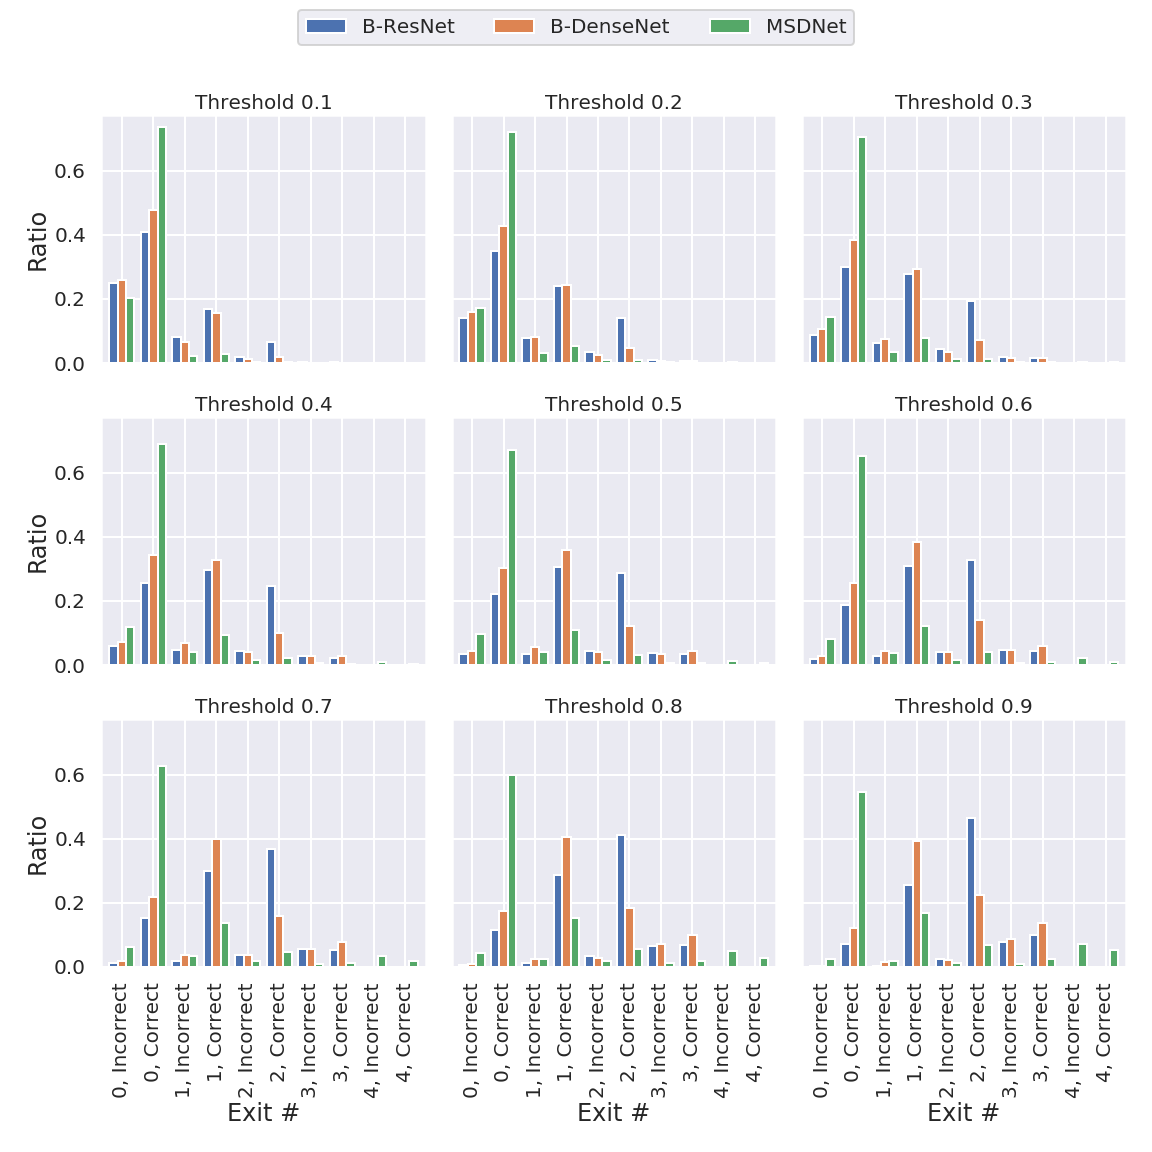
\includegraphics[width=\linewidth]{figures/threshold_plots/inference_threshold_test}
	\caption{Score-Margin Exiting}
	\label{fig:inferencethresholdtest}
\end{figure}



\section{Early Exiting vs. Conventional Inference}

Conventional versions of the \gls{resnet} and \gls{densenet} were trained on the \gls{min100}. Transfer learning was used with ImageNet weights, the model are used as a feature extractor, hence all weights were frozen and only the linear classifier was trained. The conventional models were used to compare with early exiting inference accuracy and latency on X different platforms.


\begin{longtabu}{>{\bfseries}X|X|X|X}
	\caption[Platform hardware comparison]{Platform hardware comparison of Window 10 Stationary PC and NVIDIA Jetson TX2 Edge Computer} \label{tbl:platforms} \\
	\toprule
	\rowfont{\bfseries}
	Platform & CPU & GPU & RAM  \tabularnewline
	\bottomrule
	\endfirsthead
	\multicolumn{3}{@{}l}{\textbf{\textcolor{black}{Table \ref{tbl:platforms}:}} continued}\\
	\toprule
	\rowfont{\bfseries}
	Platform & CPU & GPU & RAM  \tabularnewline
	\bottomrule
	\endhead % all the lines above this will be repeated on every page
	\bottomrule
	\multicolumn{3}{@{}l}{continued \ldots}\\
	\endfoot
	\hline
	\endlastfoot
	Windows PC & Intel i5 & NVIDIA GeForce GTX 1080, 2560 CUDA cores & 16GB \tabularnewline
	\hline
	Jetson TX2 & ARM Cortex-A57 & NVIDIA Pascal GPU, 256 CUDA cores & 8GB \tabularnewline
	\bottomrule
\end{longtabu}

The model inference characteristic on PC, see figure \ref{fig:early_exit_vs_conv}.

  \begin{figure}
  	\captionsetup[subfigure]{justification=centering}
  	\centering
  	\subfloat[Window PC\label{fig:early_exit_vs_conv}]{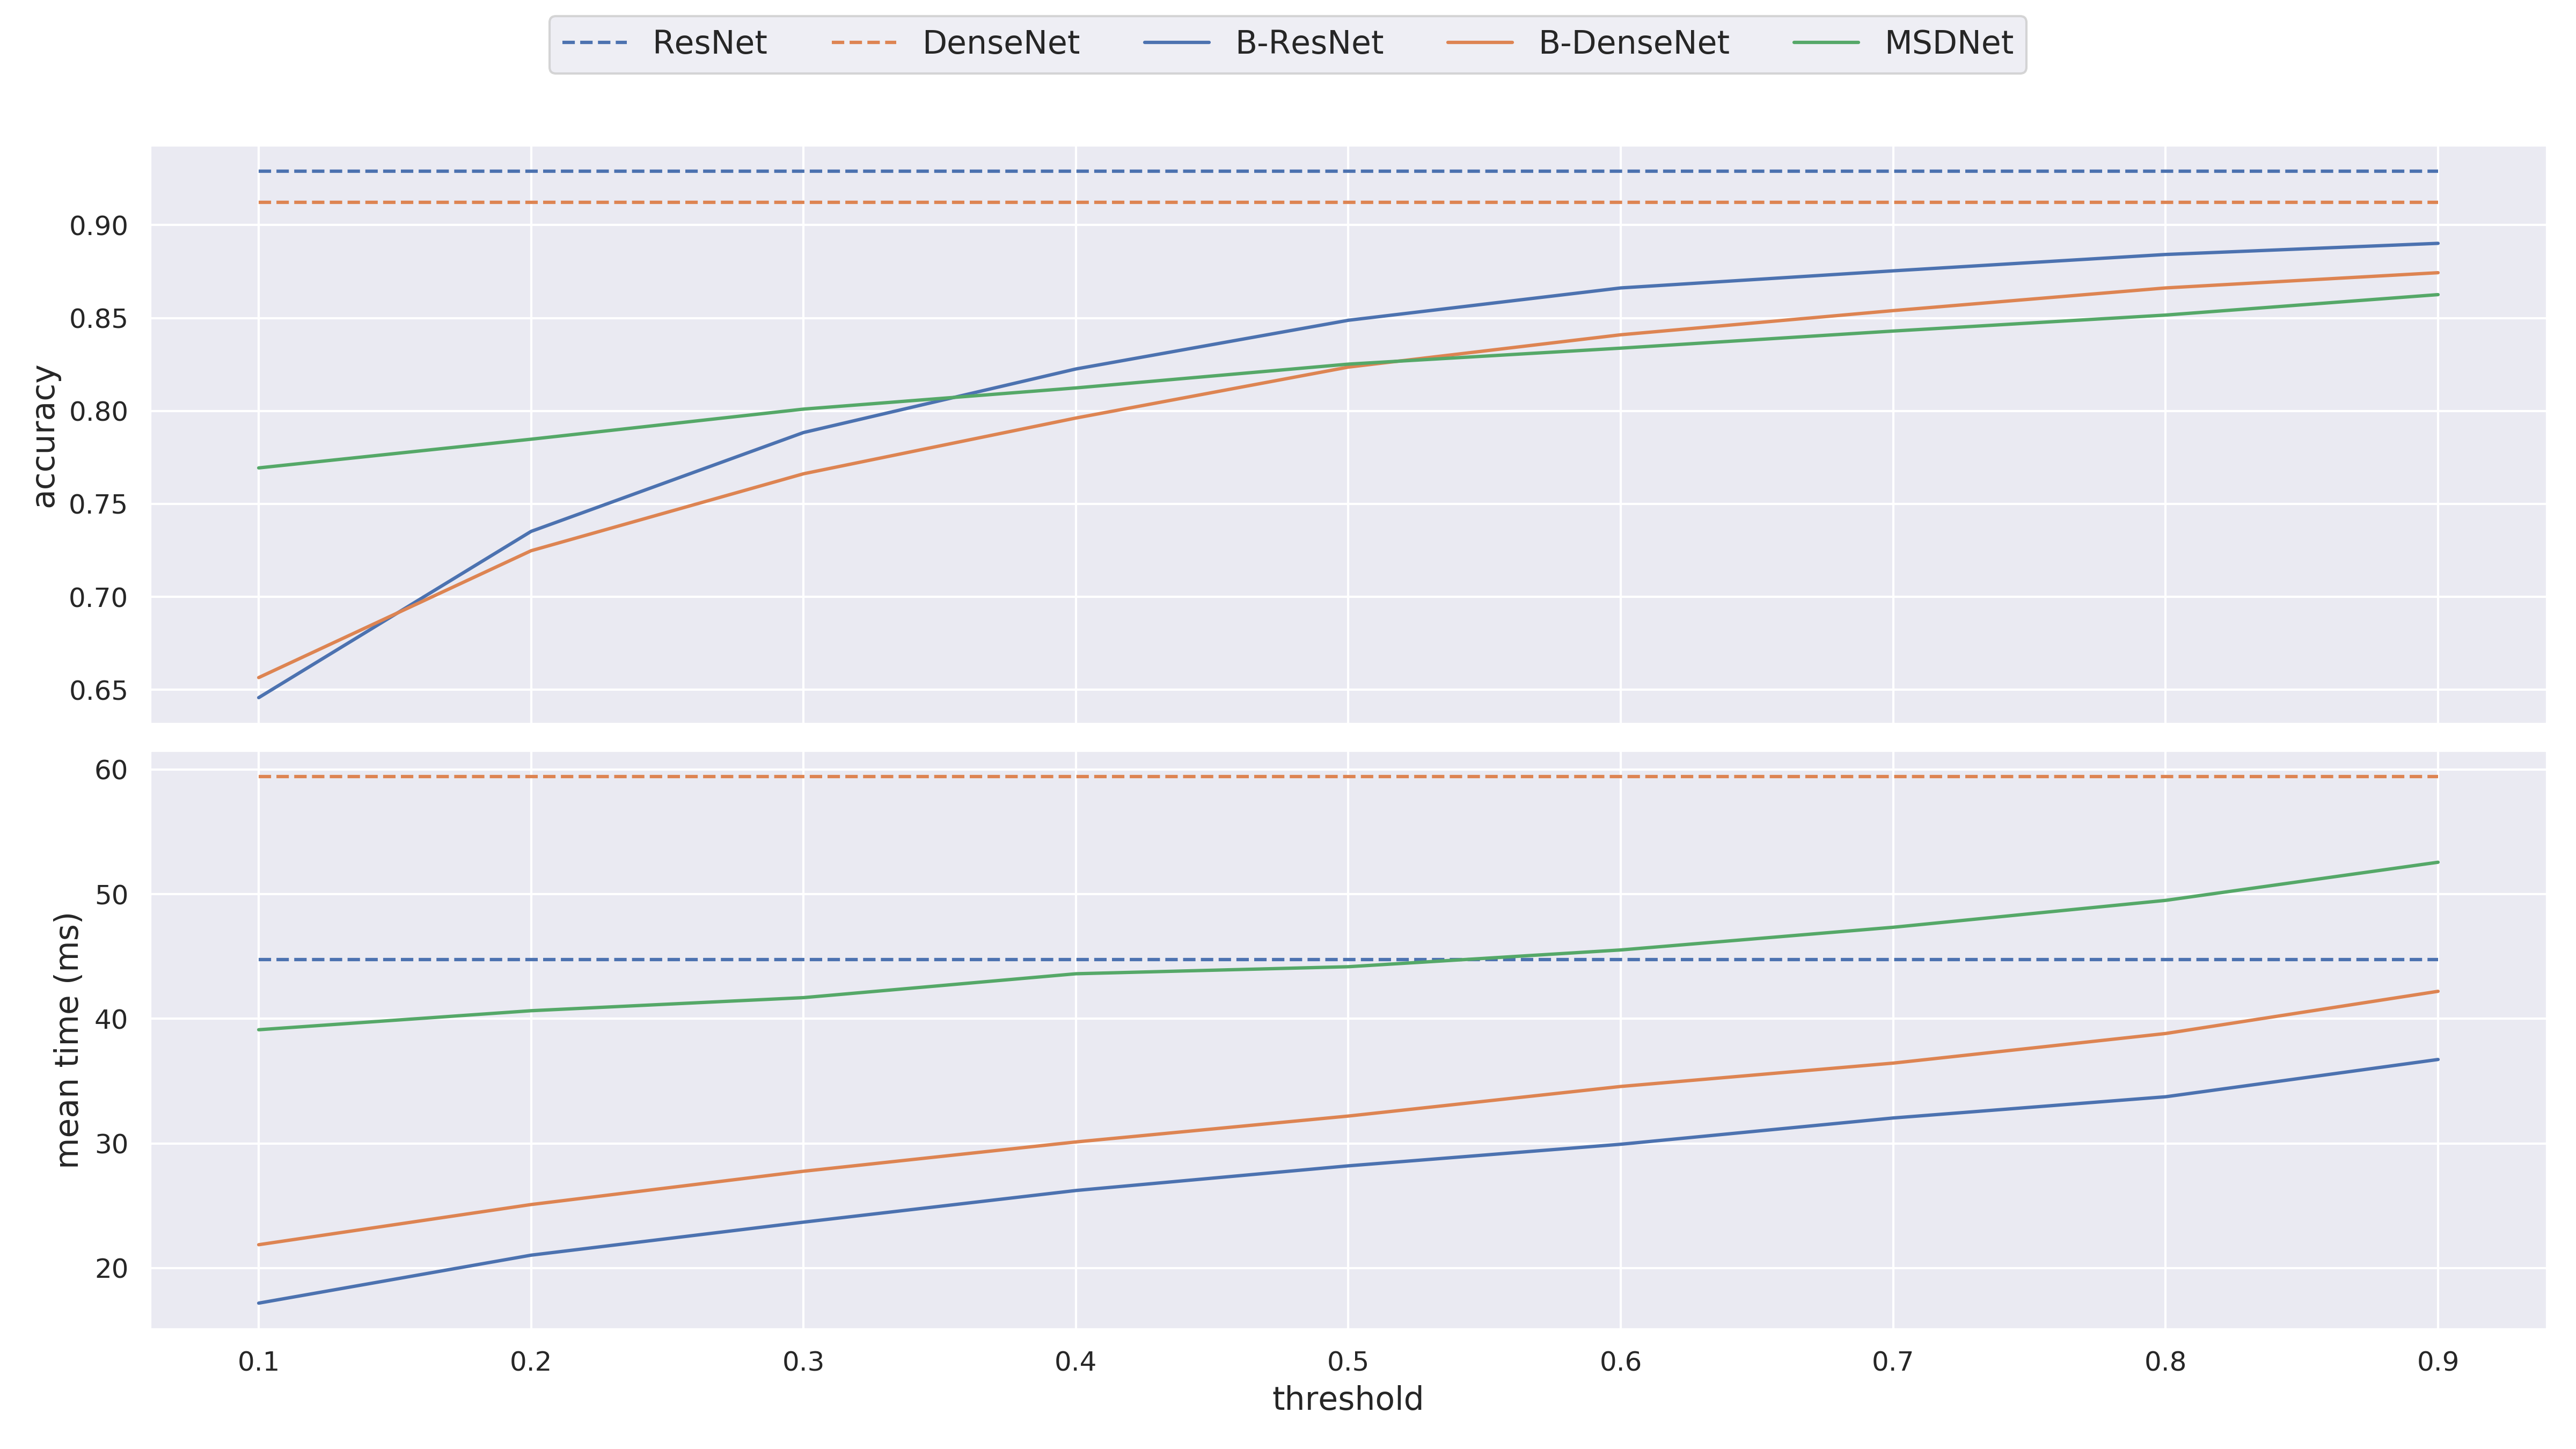
\includegraphics[width=\linewidth]{figures/threshold_plots/compare_exiting_vs_no_exiting}}
  	
  	
  \end{figure}

  \begin{figure}
	\captionsetup[subfigure]{justification=centering}
	\centering
	\subfloat[Jetson TX2\label{fig:jetson-early_exit_vs_conv}]{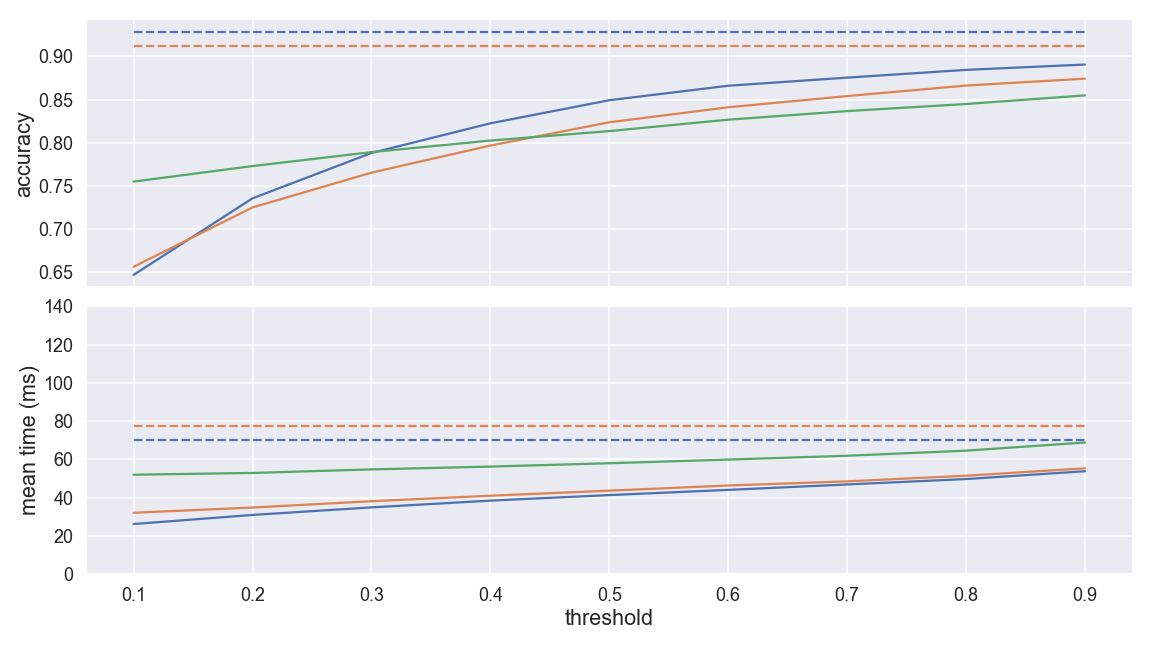
\includegraphics[width=\linewidth]{figures/threshold_plots/jetson_inference}}
\end{figure}

The figure clearly states the accuracy-latency trade-off imposed by early exiting. The conventional models are clearly more accurate, however also expectantly slower, than their more flexible exiting counterpart. B-\gls{densenet} benefits more from early exiting, when a threshold of 0.9 is chosen, it gives up 4 percentage point in accuracy and reducing inference latency by 29 \%. The B-\gls{resnet} have about the same compromise in terms of accuracy, however only a reduction of 18 \% inference latency. B-\gls{resnet} still perform better in terms of both accuracy and inference time. The \gls{resnet}. 

  \begin{figure}
	\captionsetup[subfigure]{justification=centering}
	\centering
	\subfloat[Jetson TX2 fine-grained\label{fig:jetson-fingrained}]{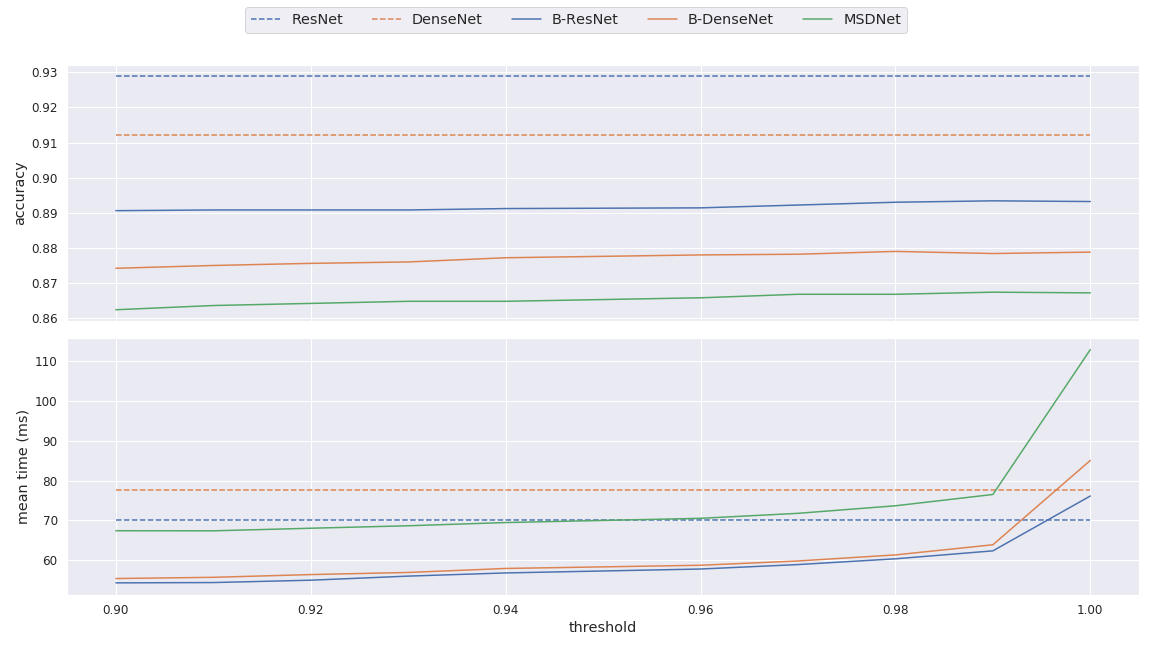
\includegraphics[width=\linewidth]{figures/threshold_plots/jetson_inference_finegrained}}
	\caption[]{}
\end{figure}

\section{Inference Time Analysis}

\begin{figure}
	\captionsetup[subfigure]{farskip=0pt,captionskip=0pt, justification=centering}
	\centering
	\subfloat{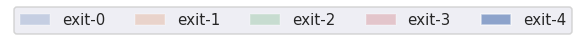
\includegraphics[width=.8\linewidth]{figures/threshold_plots/time_dist_legend}}
	\hfill
	\subfloat[Windows PC]{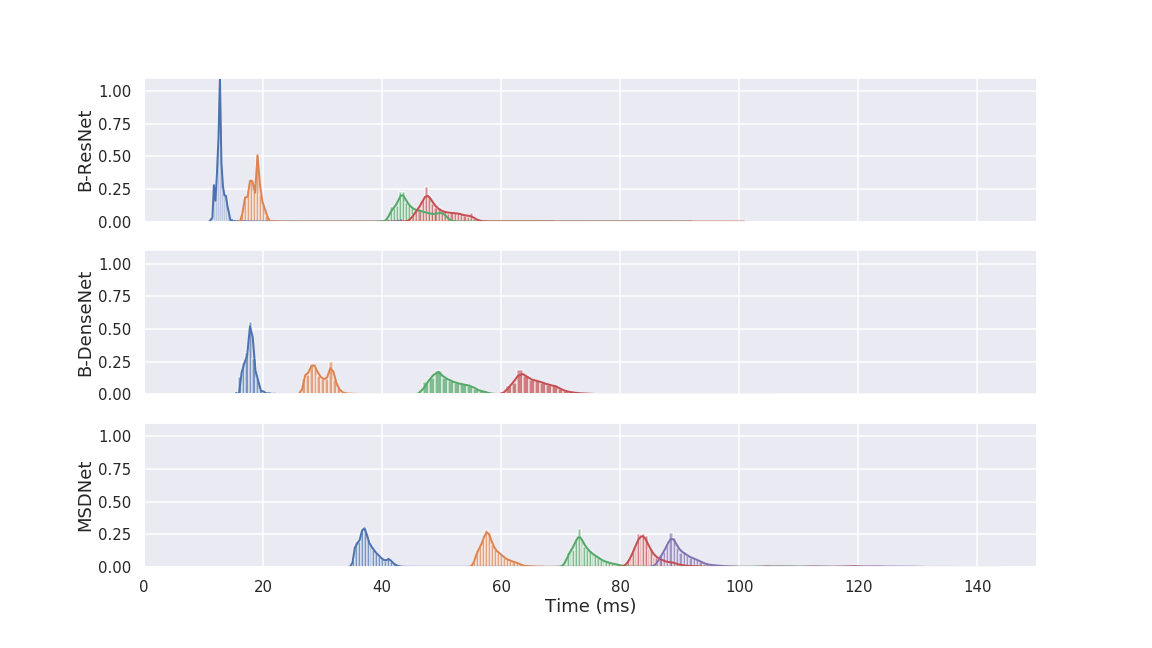
\includegraphics[width=\linewidth]{figures/threshold_plots/inference_time_distribution}}
	\hfill
	\subfloat[Jetson TX2]{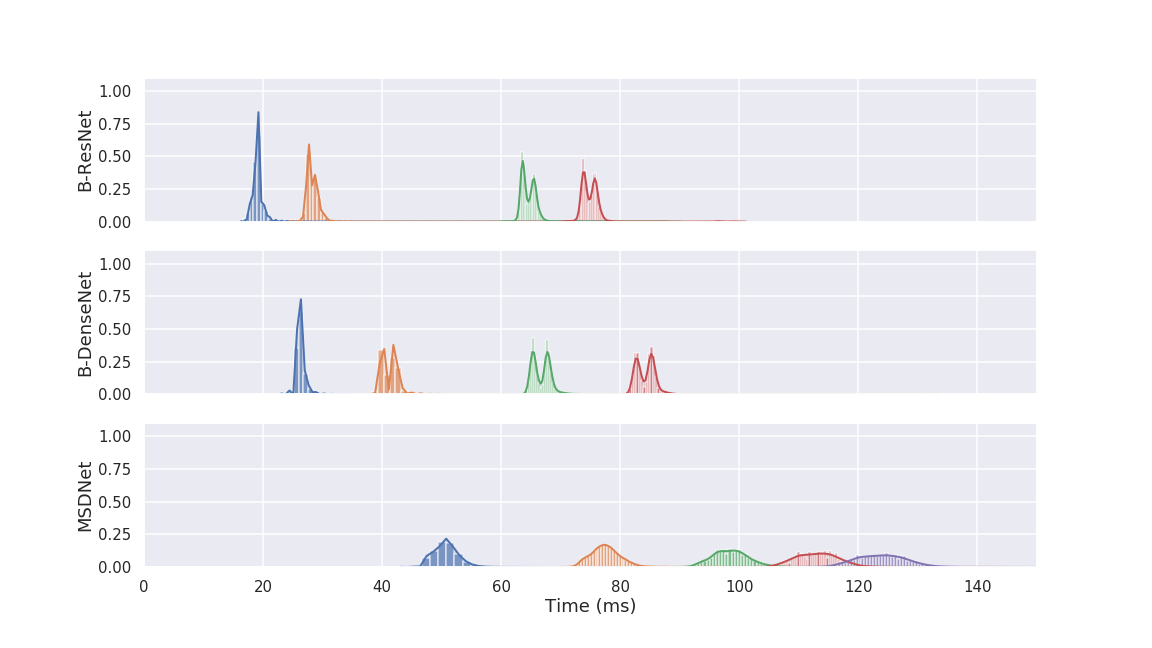
\includegraphics[width=\linewidth]{figures/threshold_plots/jetson_inference_time_distribution}}
	\caption[Inference Time Distribution]{Inference Time Distribution}
	\label{fig:inference-time-dist}
\end{figure}

\section{Time Threshold}

For time-budgeted applications, where a classification must be derived within a timed threshold. We wish to maximize the accuracy subject to this time constraint. Figure \ref{fig:time-threshold} show the model accuracy under different time constraints and on different platforms.

How to choose threshold?
If given a time threshold, what accuracy are we then able to achieve? 

\begin{figure}
	\captionsetup[subfigure]{justification=centering}
	\centering
	\subfloat[GPU Workstation]{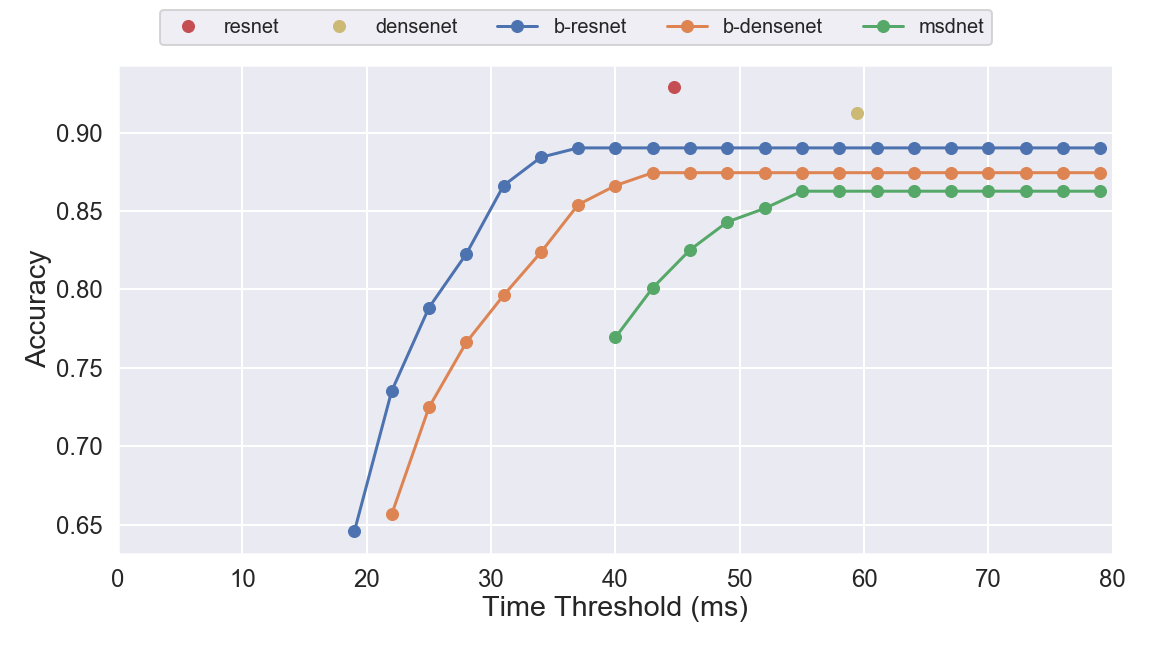
\includegraphics[width=\linewidth]{figures/threshold_plots/time_threshold_pc}}
	\hfill
	\subfloat[Jetson TX2]{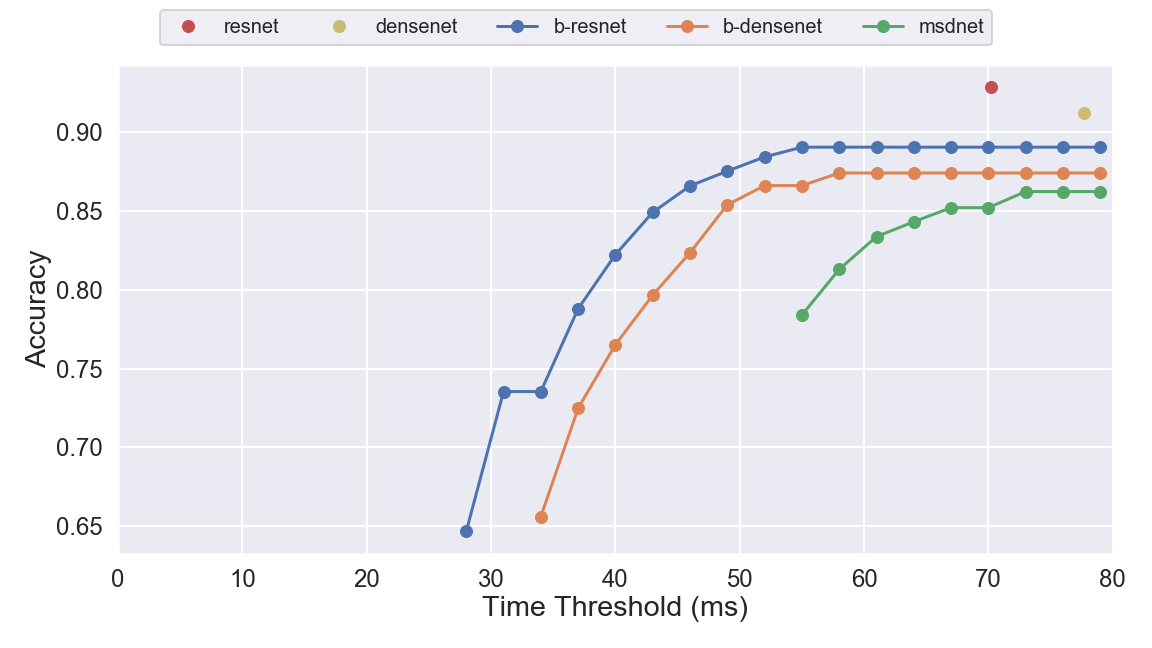
\includegraphics[width=\linewidth]{figures/threshold_plots/time_threshold_jetson}}
	\caption[Time Threshold]{Time Threshold}
	\label{fig:time-threshold}
\end{figure}

From figure \ref{fig:inference-time-dist} we know the inference time distribution for each exit on different hardwares. Given a time constraint, we can selective choose the exit with the best chance to provide a prediction within a certain time frame, similar to Edgent \cite{li_edge_2018}. The difference at first is we only focus on on-device or on-edge execution  with no collaboration, hence we do not need a regression model of the per layer execution of the \gls{dnn}. For device-only execution our only concern is the inference time on the specific hardware, a simple selection would be the exit with the largest inference time mean within the time constraint, as accuracy is monotically increasing over available time.
\begin{maxi*}
			{}{Reliabilty\sim\tau_{computation}}
	{}{}
	\addConstraint{\tau_{computation}}{\leq T}
\end{maxi*}
 In an edge-offloading scenario we must consider communication latency. If the available networking conditions are good a later exit can be chosen to improve the reliability, however in scenarios, where networking conditions are poor an earlier exit must be chosen to meet latency requirements. 
 \begin{maxi*}
 	{}{Reliabilty\sim\tau_{computation}}
 	{}{}
 	\addConstraint{(\tau_{computation}+\tau_{communication})}{\leq T}
 \end{maxi*}
The selection of exit is based on distributions of inference time, this introduces some uncertainty, as not all samples might be able to meet the latency requirement, this can be caused be derivation in compute time, congestions in the network latency or server workload. One key feature of early exiting is the ability to obtain intermediate predictions, this allow for parallel execution while offloading. The end-device might only be able to reach an early exit within the time frame, where edge server reaches a later one. However, unexpectedly no reply is received by the end-device within the time frame, then the application can use the locally obtained prediction from an earlier exit. 

Or a collaborative scheme might be used, where the end-device locally processes the algorithm up to an early exit and obtains a prediction, then it offload the rest of the execution in a cascaded manner for remote execution, still if no reply is received by the end-device within the time frame a locally obtained prediction is available albeit less reliable than if the remote prediction would have arrived in time. Multiple early exits allows for successively sending back increasingly confident and reliable predictions, at a small overhead communication, the last received prediction would then be used by the application.    
 

\section{Transport Protocol} 

Offloading tasks over the network, irregardless fully or partially requires a transport protocol. The selection is typically a choice of either \gls{tcp} or \gls{udp}. \gls{tcp} is a reliable protocol, that guarantee no losses by retransmission of lost packets. \gls{udp} on the other hand is a best-effort protocol, that accept packets loss, thus not introducing retransmission communication overhead. 


Fully offloading \gls{jpeg} compressed images for classification require no losses for human-readability. Sending intermediate features of a \gls{dnn} may not be as intolerant to losses and might be able to function with the far more lightweight \gls{udp}. In current research literature the choice of \gls{tcp} seems given in advance.  

In this experiment the \gls{tcp} transmission time and retransmission rate is investigated under different communication environments. 

\begin{figure}
	\centering
	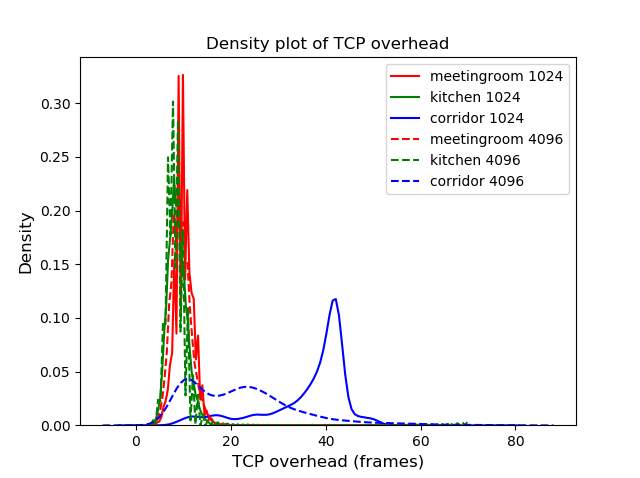
\includegraphics[width=\linewidth]{figures/tcp/tcpoverhead}
	\caption[TCP retransmission overhead]{TCP retransmission overhead}
\end{figure}






% \section{\acrlong{ddnn}}

\gls{ddnn} is an early exit framework proposed by \citet{teerapittayanon_distributed_2017} as their fllow-up on BranchyNet \cite{teerapittayanon_branchynet:_2016} extending the early exit model into a distributed system over cloud, edge and end devices.

This thesis implements the \gls{ddnn} framework, however extending the device model to implement \cite{sandler_mobilenetv2:_2018} and edge model to implement ResNet152 \cite{he_deep_2015} and train on a more complex dataset, Pascal VOC \cite{everingham_pascal_2010}. 